\documentclass[hide notes,intlimits]{beamer}


\mode<presentation>
{
  \usetheme{UAFshade}
  \setbeamercovered{transparent}
}

% load packages
\usepackage{multimedia}
\usepackage{animate}
\usepackage[english]{babel}
\usepackage[latin1]{inputenc}
\usepackage[T1]{fontenc}
\usepackage{lmodern}
\usepackage[multidot]{grffile}
\usepackage[amssymb]{SIunits}

\usepackage{tikz}
\usetikzlibrary{shapes,arrows,shadows, calc}

\usepackage{pgfpages}
\setbeamertemplate{note page}[plain]
\setbeameroption{show notes on second screen=right}


\definecolor{dark red}{HTML}{E41A1C}
\definecolor{dark green}{HTML}{4DAF4A}
\definecolor{dark violet}{HTML}{984EA3}
\definecolor{dark blue}{HTML}{084594}
\definecolor{dark orange}{HTML}{FF7F00}
\definecolor{white}{HTML}{FFFFFF}
\definecolor{light blue}{HTML}{377EB8}
\definecolor{light red}{HTML}{FB9A99}
\definecolor{light violet}{HTML}{CAB2D6}

\definecolor{uaf red}{HTML}{E41A1C}
\definecolor{uaf blue}{HTML}{377EB8}
\definecolor{uaf green}{HTML}{4DAF4A}
\definecolor{uaf violet}{HTML}{984EA3}
\definecolor{uaf orange}{HTML}{FF7F00}
\setbeamercolor{boxed}{fg=black,bg=uaf yellow}


% Define block styles
\tikzstyle{initialization} = [ellipse, draw, 
    text badly centered, draw=dark violet,
        % The filling: 
        top color=white, 
        bottom color=dark violet]
\tikzstyle{initialization faded} = [ellipse, draw, 
    text badly centered, draw=dark violet!50,
        % The filling: 
        top color=white, 
        bottom color=dark violet!25]
\tikzstyle{hindcast} = [ellipse, draw,
    text badly centered, rounded corners,draw=dark orange,
        % The filling: 
        top color=white, 
        bottom color=dark orange]
\tikzstyle{hindcast faded} = [ellipse, draw,
    text badly centered, rounded corners,draw=dark orange!50,
        % The filling: 
        top color=white, 
        bottom color=dark orange!25]
\tikzstyle{forecast} = [ellipse, draw,
    text badly centered, rounded corners,draw=dark blue,
        % The filling: 
        top color=white, 
        bottom color=dark blue]
\tikzstyle{forecast faded} = [ellipse, draw,
    text badly centered, rounded corners,draw=dark blue!50,
        % The filling: 
        top color=white, 
        bottom color=dark blue!50]
\tikzstyle{arrow line} = [draw, -latex']
\tikzstyle{line} = [draw]



\graphicspath{{figures/}}

\setbeamerfont{caption}{size=\scriptsize}

% code adapted from http://tex.stackexchange.com/a/11483/3954

% some parameters for customization
\def\shadowshift{3pt,-3pt}
\def\shadowradius{6pt}

\colorlet{innercolor}{black!60}
\colorlet{outercolor}{gray!05}

% this draws a shadow under a rectangle node
\newcommand\drawshadow[1]{
    \begin{pgfonlayer}{shadow}
        \shade[outercolor,inner color=innercolor,outer color=outercolor] ($(#1.south west)+(\shadowshift)+(\shadowradius/2,\shadowradius/2)$) circle (\shadowradius);
        \shade[outercolor,inner color=innercolor,outer color=outercolor] ($(#1.north west)+(\shadowshift)+(\shadowradius/2,-\shadowradius/2)$) circle (\shadowradius);
        \shade[outercolor,inner color=innercolor,outer color=outercolor] ($(#1.south east)+(\shadowshift)+(-\shadowradius/2,\shadowradius/2)$) circle (\shadowradius);
        \shade[outercolor,inner color=innercolor,outer color=outercolor] ($(#1.north east)+(\shadowshift)+(-\shadowradius/2,-\shadowradius/2)$) circle (\shadowradius);
        \shade[top color=innercolor,bottom color=outercolor] ($(#1.south west)+(\shadowshift)+(\shadowradius/2,-\shadowradius/2)$) rectangle ($(#1.south east)+(\shadowshift)+(-\shadowradius/2,\shadowradius/2)$);
        \shade[left color=innercolor,right color=outercolor] ($(#1.south east)+(\shadowshift)+(-\shadowradius/2,\shadowradius/2)$) rectangle ($(#1.north east)+(\shadowshift)+(\shadowradius/2,-\shadowradius/2)$);
        \shade[bottom color=innercolor,top color=outercolor] ($(#1.north west)+(\shadowshift)+(\shadowradius/2,-\shadowradius/2)$) rectangle ($(#1.north east)+(\shadowshift)+(-\shadowradius/2,\shadowradius/2)$);
        \shade[outercolor,right color=innercolor,left color=outercolor] ($(#1.south west)+(\shadowshift)+(-\shadowradius/2,\shadowradius/2)$) rectangle ($(#1.north west)+(\shadowshift)+(\shadowradius/2,-\shadowradius/2)$);
        \filldraw ($(#1.south west)+(\shadowshift)+(\shadowradius/2,\shadowradius/2)$) rectangle ($(#1.north east)+(\shadowshift)-(\shadowradius/2,\shadowradius/2)$);
    \end{pgfonlayer}
}

% create a shadow layer, so that we don't need to worry about overdrawing other things
\pgfdeclarelayer{shadow} 
\pgfsetlayers{shadow,main}

\newsavebox\mybox
\newlength\mylen

\newcommand\shadowimage[2][]{%
\setbox0=\hbox{\includegraphics[#1]{#2}}
\setlength\mylen{\wd0}
\ifnum\mylen<\ht0
\setlength\mylen{\ht0}
\fi
\divide \mylen by 120
\def\shadowshift{\mylen,-\mylen}
\def\shadowradius{\the\dimexpr\mylen+\mylen+\mylen\relax}
\begin{tikzpicture}
\node[anchor=south west,inner sep=0] (image) at (0,0) {\includegraphics[#1]{#2}};
\drawshadow{image}
\end{tikzpicture}}

\newcommand\shadowimagec[3][]{%
\setbox0=\hbox{\includegraphics<#1>[#2]{#3}}
\setlength\mylen{\wd0}
\ifnum\mylen<\ht0
\setlength\mylen{\ht0}
\fi
\divide \mylen by 120
\def\shadowshift{\mylen,-\mylen}
\def\shadowradius{\the\dimexpr\mylen+\mylen+\mylen\relax}
\begin{tikzpicture}
\node[anchor=south west,inner sep=0] (image) at (0,0) {\includegraphics<#1>[#2]{#3}};
\drawshadow{image}
\end{tikzpicture}}


\newenvironment{transbox}[1][]{%
\begin{tikzpicture}
\node[drop shadow,rounded corners,text width=\textwidth,fill=white, fill opacity=#1,text opacity=1] \bgroup
}{
\egroup;\end{tikzpicture}} 

\newenvironment{transbox-tight}{%
\begin{tikzpicture}
\node[drop shadow,rounded corners,fill=uaf yellow, fill opacity=0.75,text opacity=1] \bgroup
}{
\egroup;\end{tikzpicture}} 


% title page
\title[] % (optional, use only with long paper titles)
{Glaciers: The Biggest Losers}



\author[Aschwanden] % (optional, use only with lots of authors)
{Andy Aschwanden}
% - Give the names in the same order as the appear in the paper.
% - Use the \inst{?} command only if the authors have different
%   affiliation.

\institute[Geophysical Institute] % (optional, but mostly needed)
{Geophysical Institute}
% - Use the \inst command only if there are several affiliations.
% - Keep it simple, no one is interested in your street address.


\date{}

\begin{document}

% define what is shown at the beginning of each section
\AtBeginSection[]
{
  \begin{frame}<handout:0>
    \frametitle{Outline}
   \tableofcontents[currentsection,subsectionstyle=hide/hide/hide]
  \end{frame}
}

% define what is shown at the beginning of each subsection
\AtBeginSubsection[]
{
 \begin{frame}<beamer>
  \frametitle{Outline}
   \tableofcontents[currentsection,currentsubsection]
 \end{frame}
}


\setbeamertemplate{background canvas}
  {
     \tikz{\node[inner sep=0pt,opacity=1.] {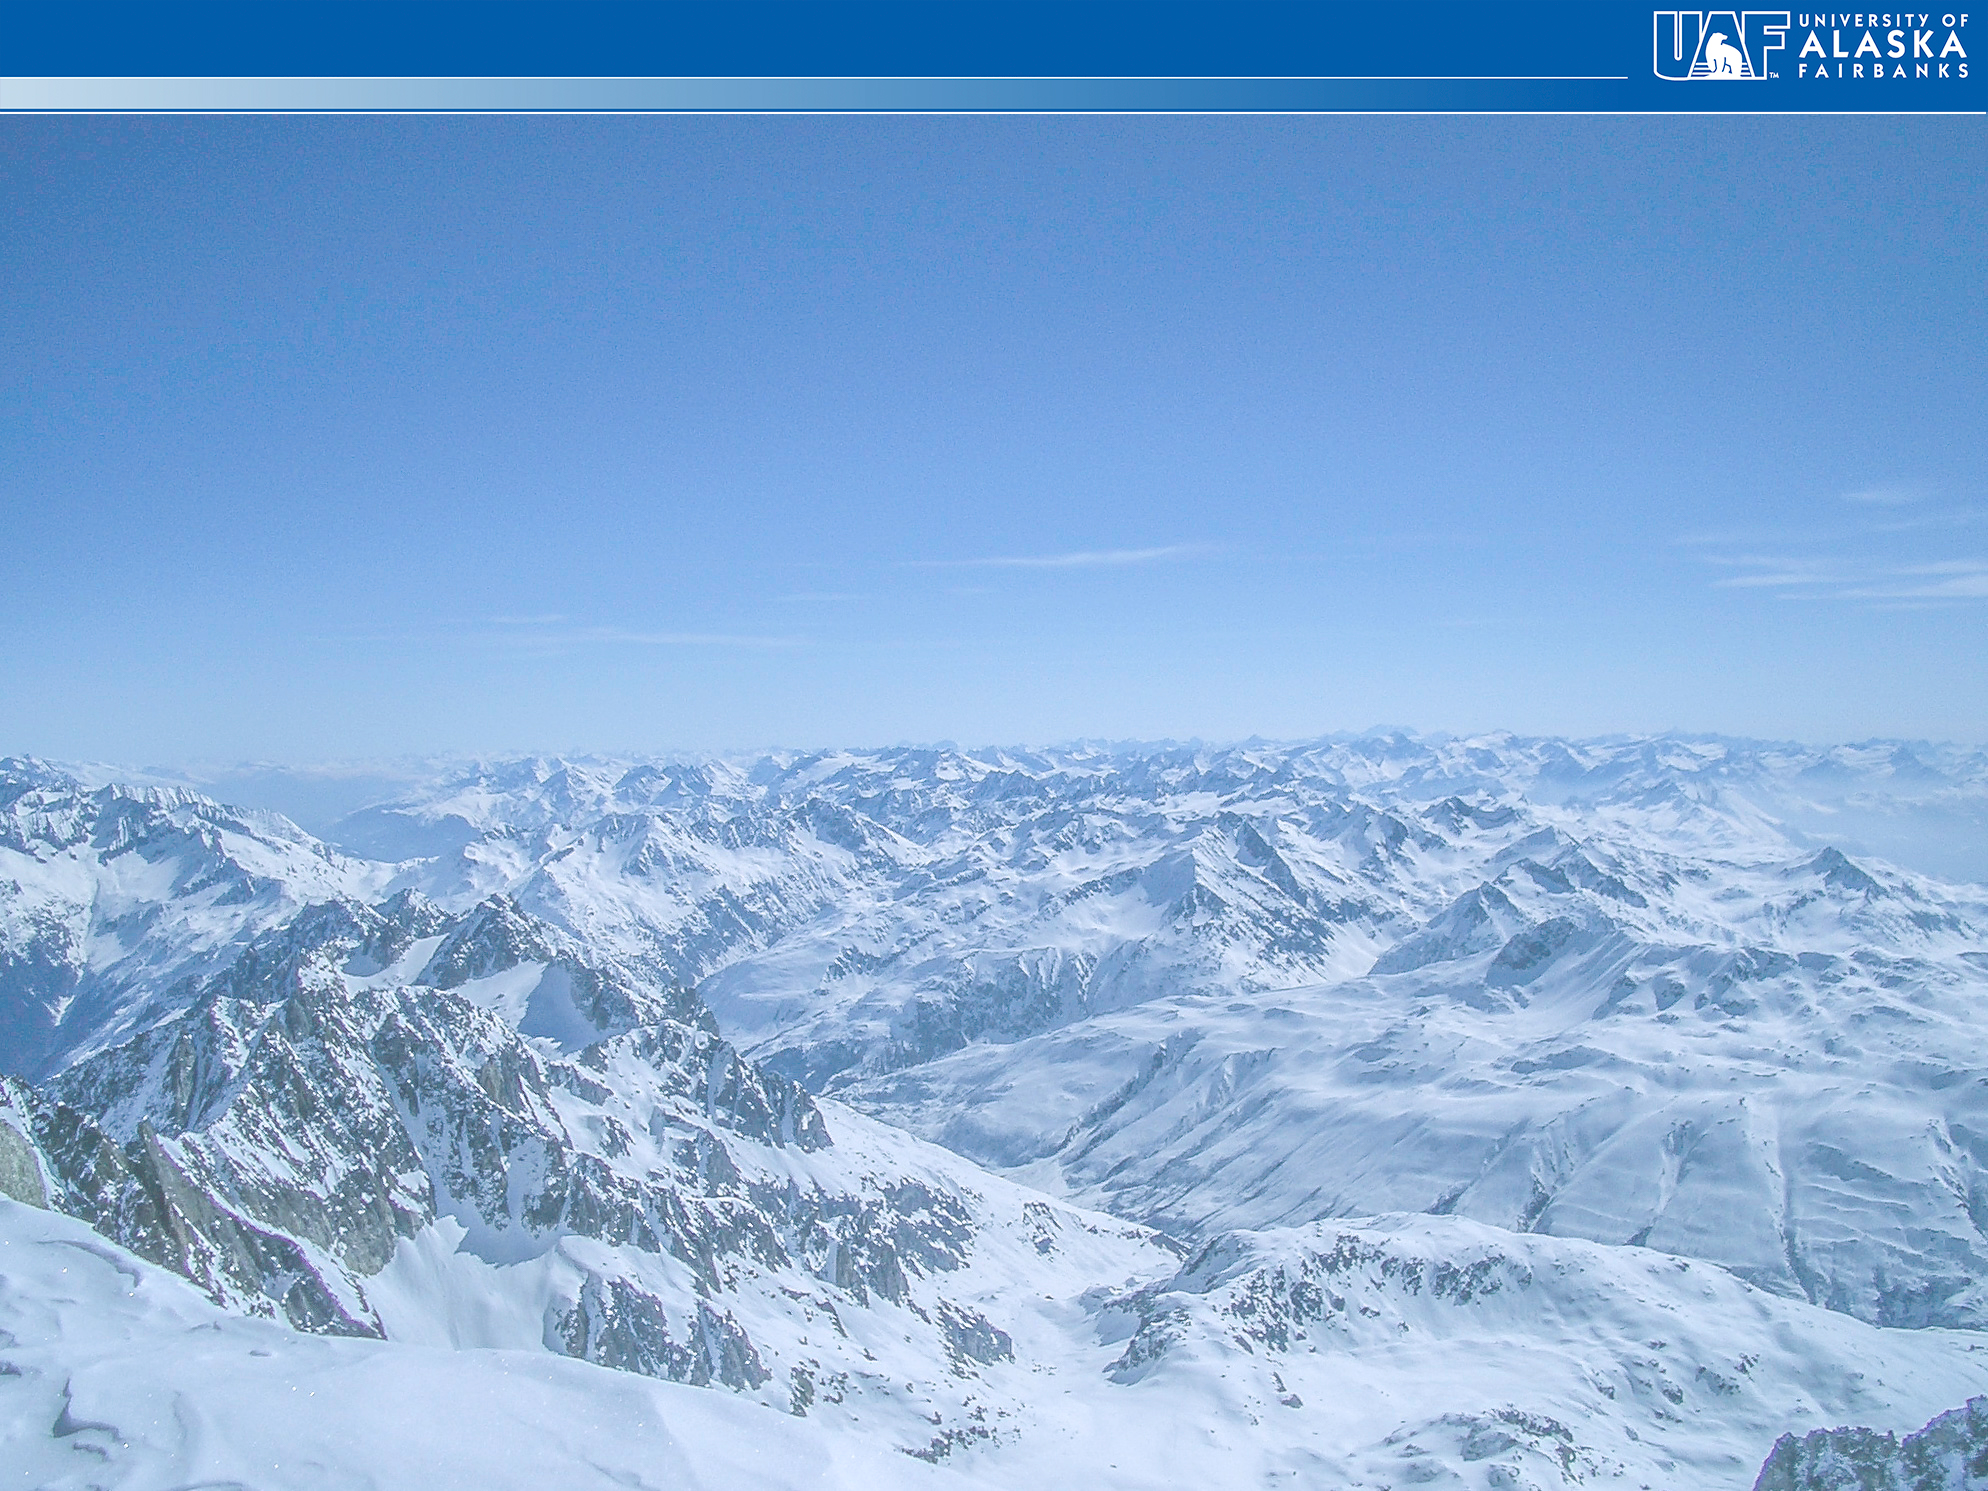
\includegraphics[width=\paperwidth]{galenstock_bg}};}
}


% insert titlepage
\begin{frame}
  \titlepage
  \note[item]{Who has ever seen a glacier?}
  \note[item]{Who has ever set foot on a glacier?}
  \note[item]{The picture here shows the view from on of my favorite places near}
  \note[item]{where I grew up}
\end{frame}

\setbeamertemplate{background canvas}
  {
} 


\setbeamertemplate{background canvas}
  {
     \tikz{\node[inner sep=0pt,opacity=1.] {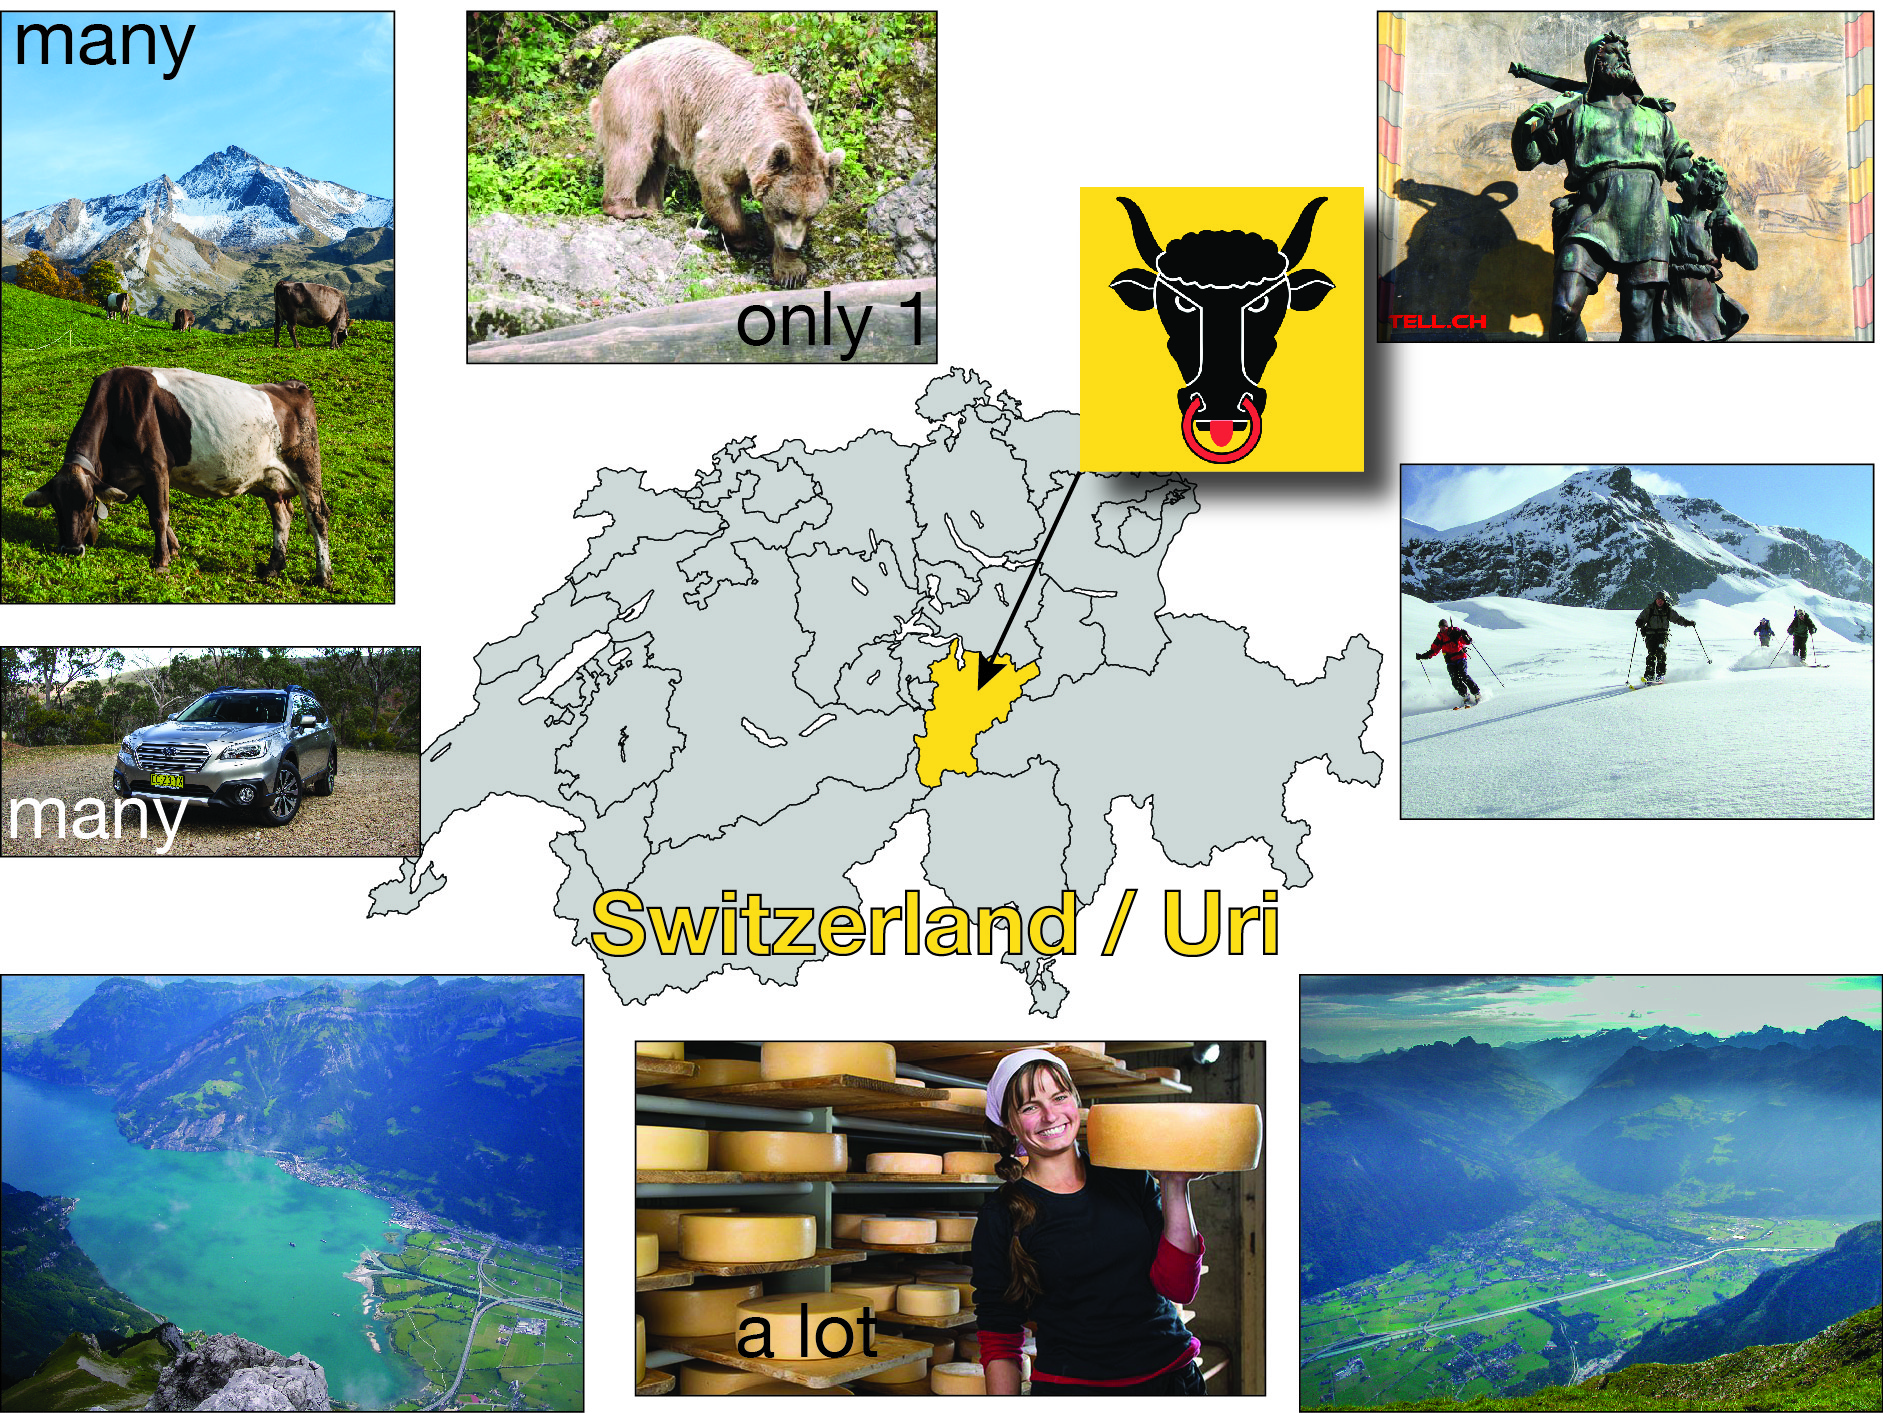
\includegraphics[width=\paperwidth]{uri-collage}};}
}

\begin{frame}[plain]
  \note[item]{I grew up in the heart of Switzerland, in the Kanton Uri---a Kanton is the equivalent to a State}
  \note[item]{Like Alaska, we have many Subarus}
  \note[item]{True to the stereotype, we have many cows in Uri and produce a lot of good cheese}
  \note[item]{Last year we had on bear roaming through Uri, which gave it some Alaska-feel}
  \note[item]{The last bear was shot in Uri in 1820 and you can still see the claws mounted to a house}
  \note[item]{According to legend, William Tell was born in Uri, who freed us from the Austrian oppression in 1291}
  \note[item]{But first and foremost have a lot of mountains to climb and to ski}
\end{frame}

\setbeamertemplate{background canvas}
{
  \tikz{\node[inner sep=0pt,opacity=1.] {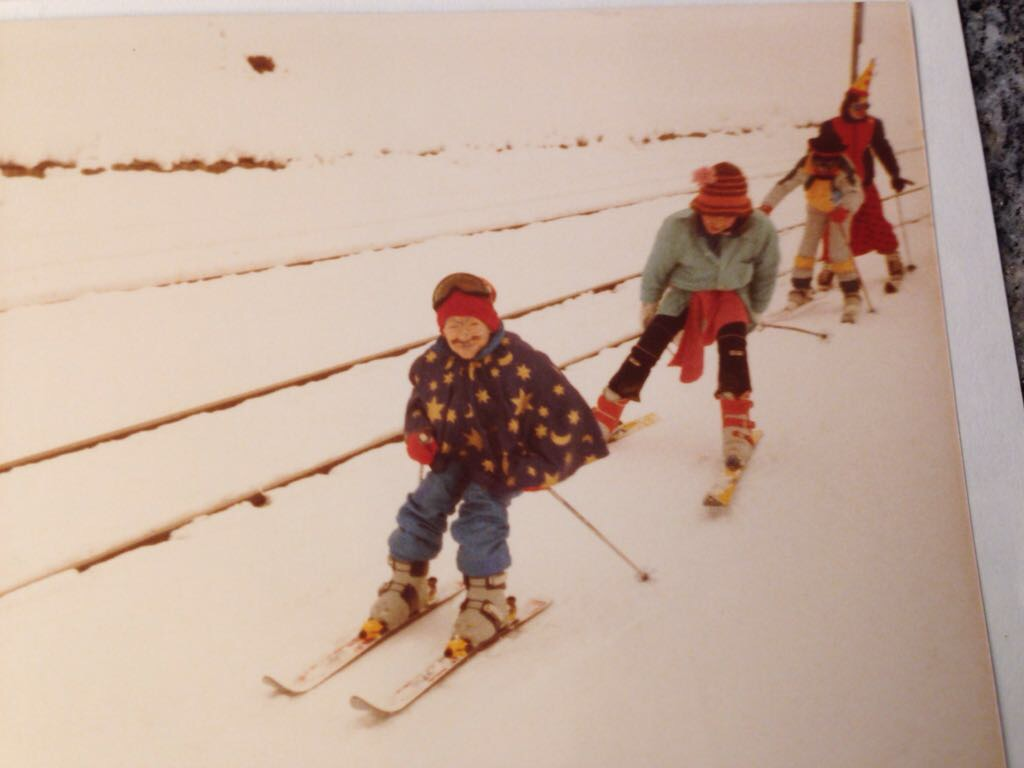
\includegraphics[width=\paperwidth]{andy-ski}};}
}

\begin{frame}[plain]
  \note[item]{So no surprise}
  \note[item]{I grew up on skis, I learned to downhill ski right after learning to walk}
  \note[item]{In Switzerland ``skiing'' always means downhill skiing, unlike here in Fairbanks where skiing usually means XC skiing}
\end{frame}



\setbeamertemplate{background canvas}
{
  \tikz{\node[inner sep=0pt,opacity=1.] {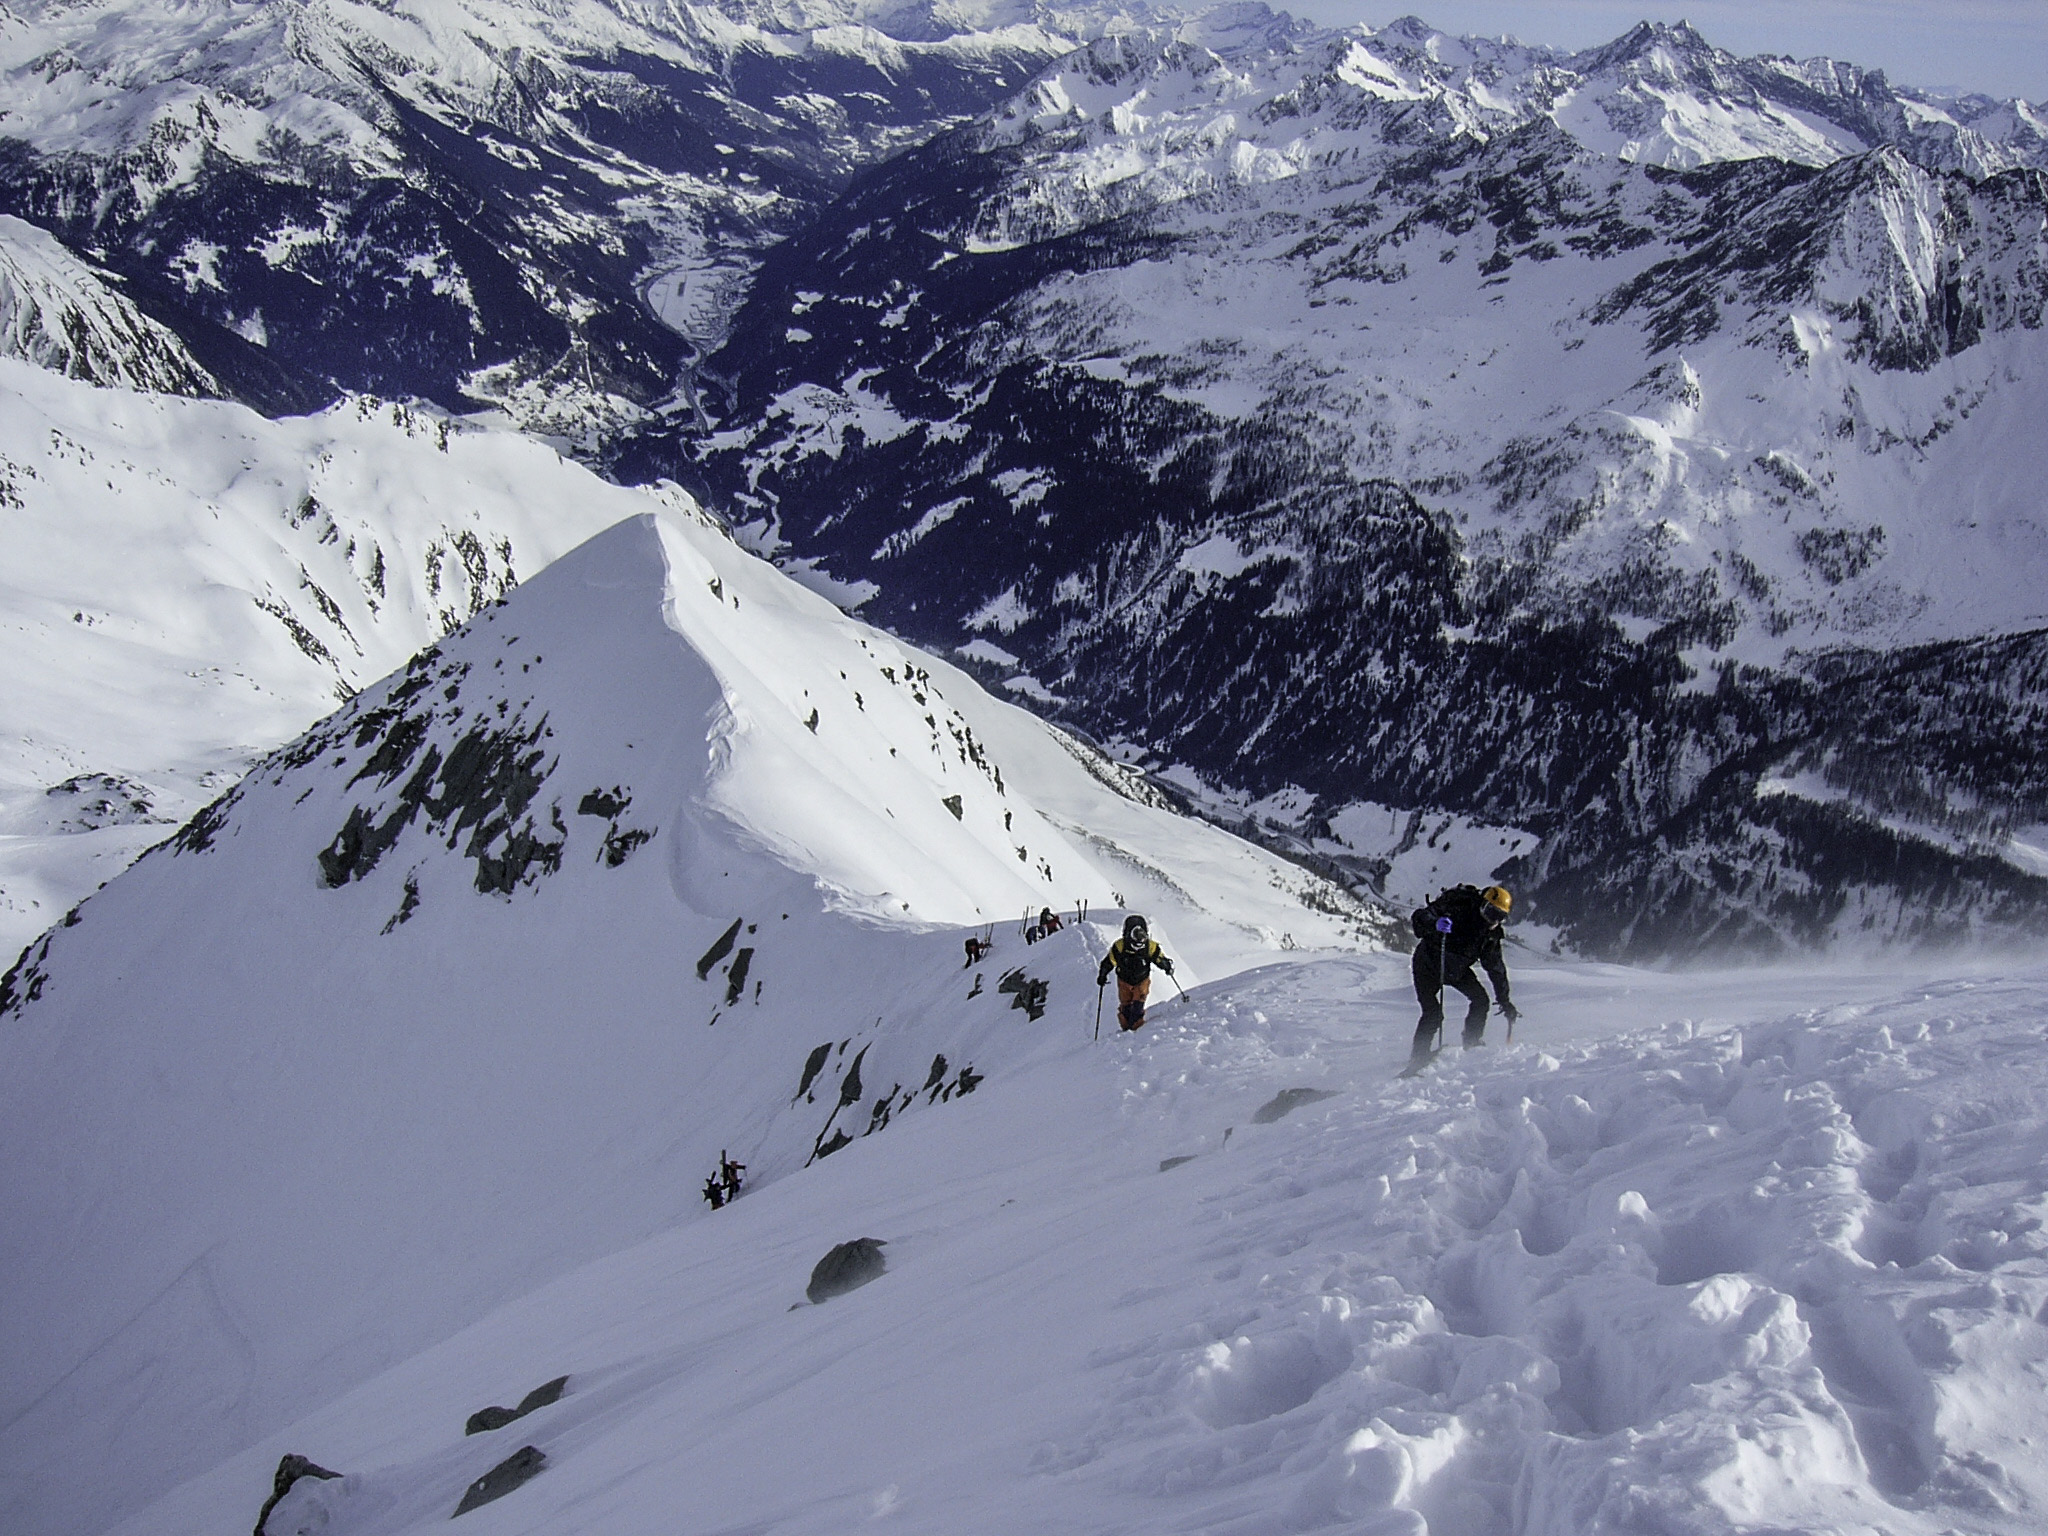
\includegraphics[width=\paperwidth]{ski-climb}};}
}

\begin{frame}[plain]
  \note[item]{When I was a bit older, I became tired of waiting for the next gondola}
  \note[item]{so started with ski mountaineering}
  \note[item]{and while spending my weekends in the mountains, I started to notice change}
\end{frame}

\setbeamertemplate{background canvas}
{
  \tikz{\node[inner sep=0pt,opacity=1.] {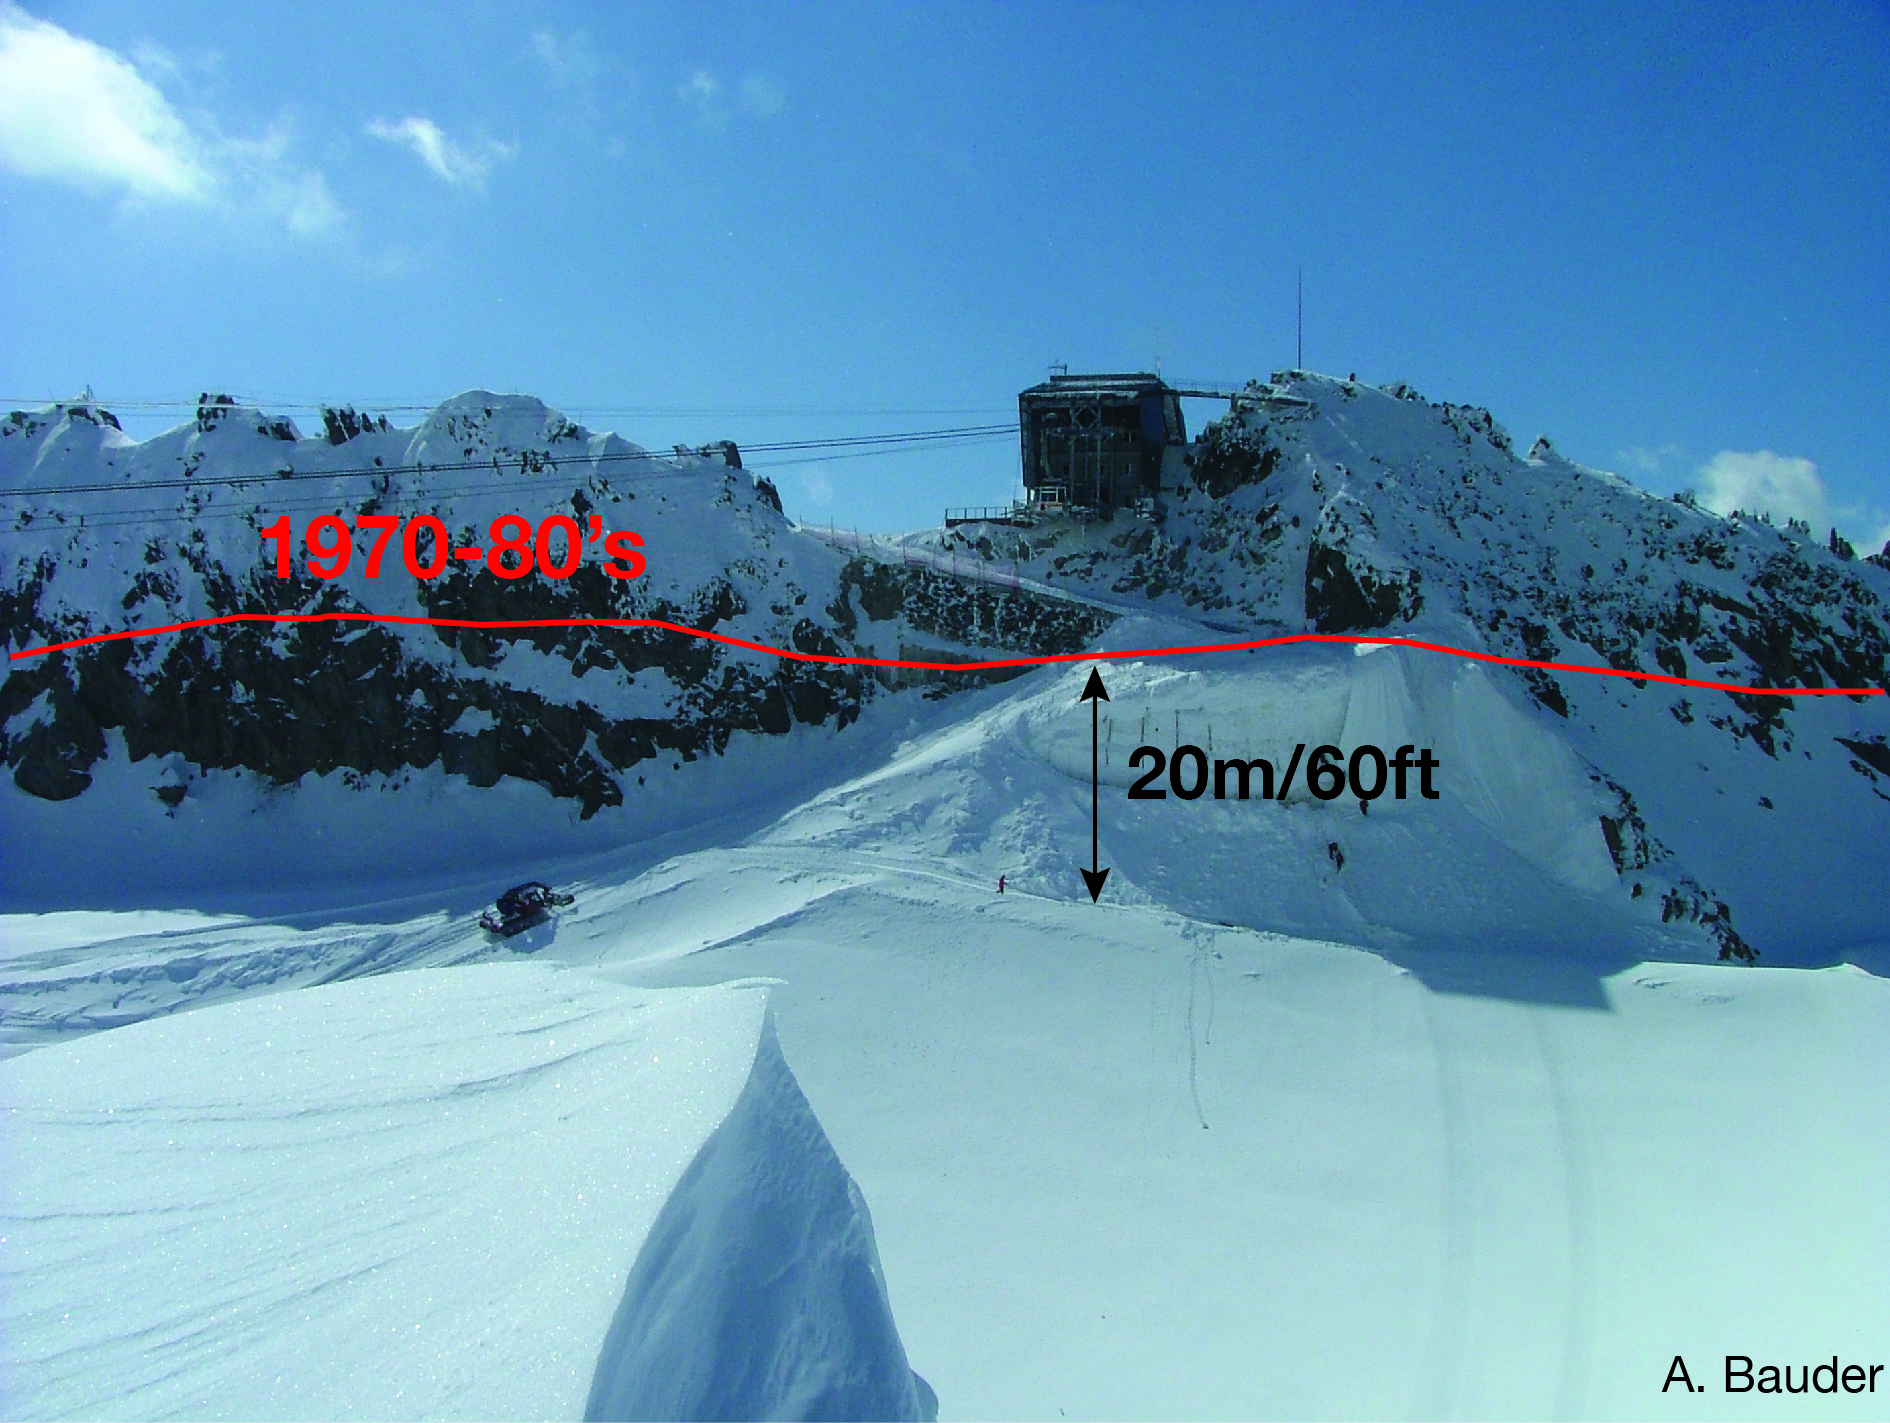
\includegraphics[width=\paperwidth]{gurschen-bauder}};}
}


\begin{frame}[plain]
  \note[item]{For example, when I was little we got out of the gondola}
  \note[item]{and we started to ski right on the glacier}
  \note[item]{However, in the past 2 or 3 decades, the glacier thinned by 20\,m or more}
  \note[item]{To get skiers on the glacier, they have to build a ramp out of snow every year}
  \note[item]{This is quite labor intensive and requires a lot of gas}
  \note[item]{Now, every spring ski patrol covers the ramp with a white tarp to preserve as much as possible}
  \note[item]{for the next winter}
  \note[item]{I asked myself: Are glaciers melting only where I grew up or is there more to it?}
  \note[item]{so, to answer this, I decided to study glaciers and climate}
  \note[item]{but also it sounded like fun to study something that I can ski on\ldots}
  \note[item]{So during the rest of talk, I would like to give you my perspective of glaciers and glacier change}
  \note[item]{I will tell you about the health of Alaska's glaciers and we glacilogists are so concerned about WAIS}
\end{frame}
  

\setbeamertemplate{background canvas}
{
} 


% \begin{frame}
%   \begin{itemize}
%     \item Presently, 10 percent of land area on Earth is covered with glacial ice, including glaciers, ice caps, and the ice sheets of Greenland and Antarctica. Glacierized areas cover over 15 million square kilometers (5.8 million square miles).
%     \item Glaciers store about 75 percent of the world's fresh water.
%     \item During the maximum point of the last ice age, glaciers covered about 32 percent of the total land area.
% \item size of AK: 663,268 sq mi (1,717,856 km2), glaciers: 87,000 sq km
%   \end{itemize}
% \end{frame}

% \begin{frame}
% \begin{itemize}
% \item what do we use glaciers for?
% \item contain 75\% of the world's fresh water
% \item electricity, hydrodam, summer
% \end{itemize}
% \end{frame}

% \begin{frame}{Glaciers Flow}
% \begin{itemize}
% \item what do we use glaciers for?
% \item contain 75\% of the world's fresh water
% \item electricity, hydrodam, summer
% \end{itemize}
% \end{frame}


% \begin{frame}{Witnessing Glacier Change in Switzerland}
%       \begin{figure}
%         \only<1>{1994\\}
%         \only<2>{2006\\}
%         \includegraphics<1>[width=\textwidth]{steigletscher-repeat-1994}
%         \includegraphics<2>[width=\textwidth]{steigletscher-repeat-2006} 
%         {\\ \footnotesize{www.swisseduc.ch}}
%       \end{figure}
% \end{frame}

\setbeamertemplate{background canvas}
{
  \tikz{\node[inner sep=0pt,opacity=0.5] {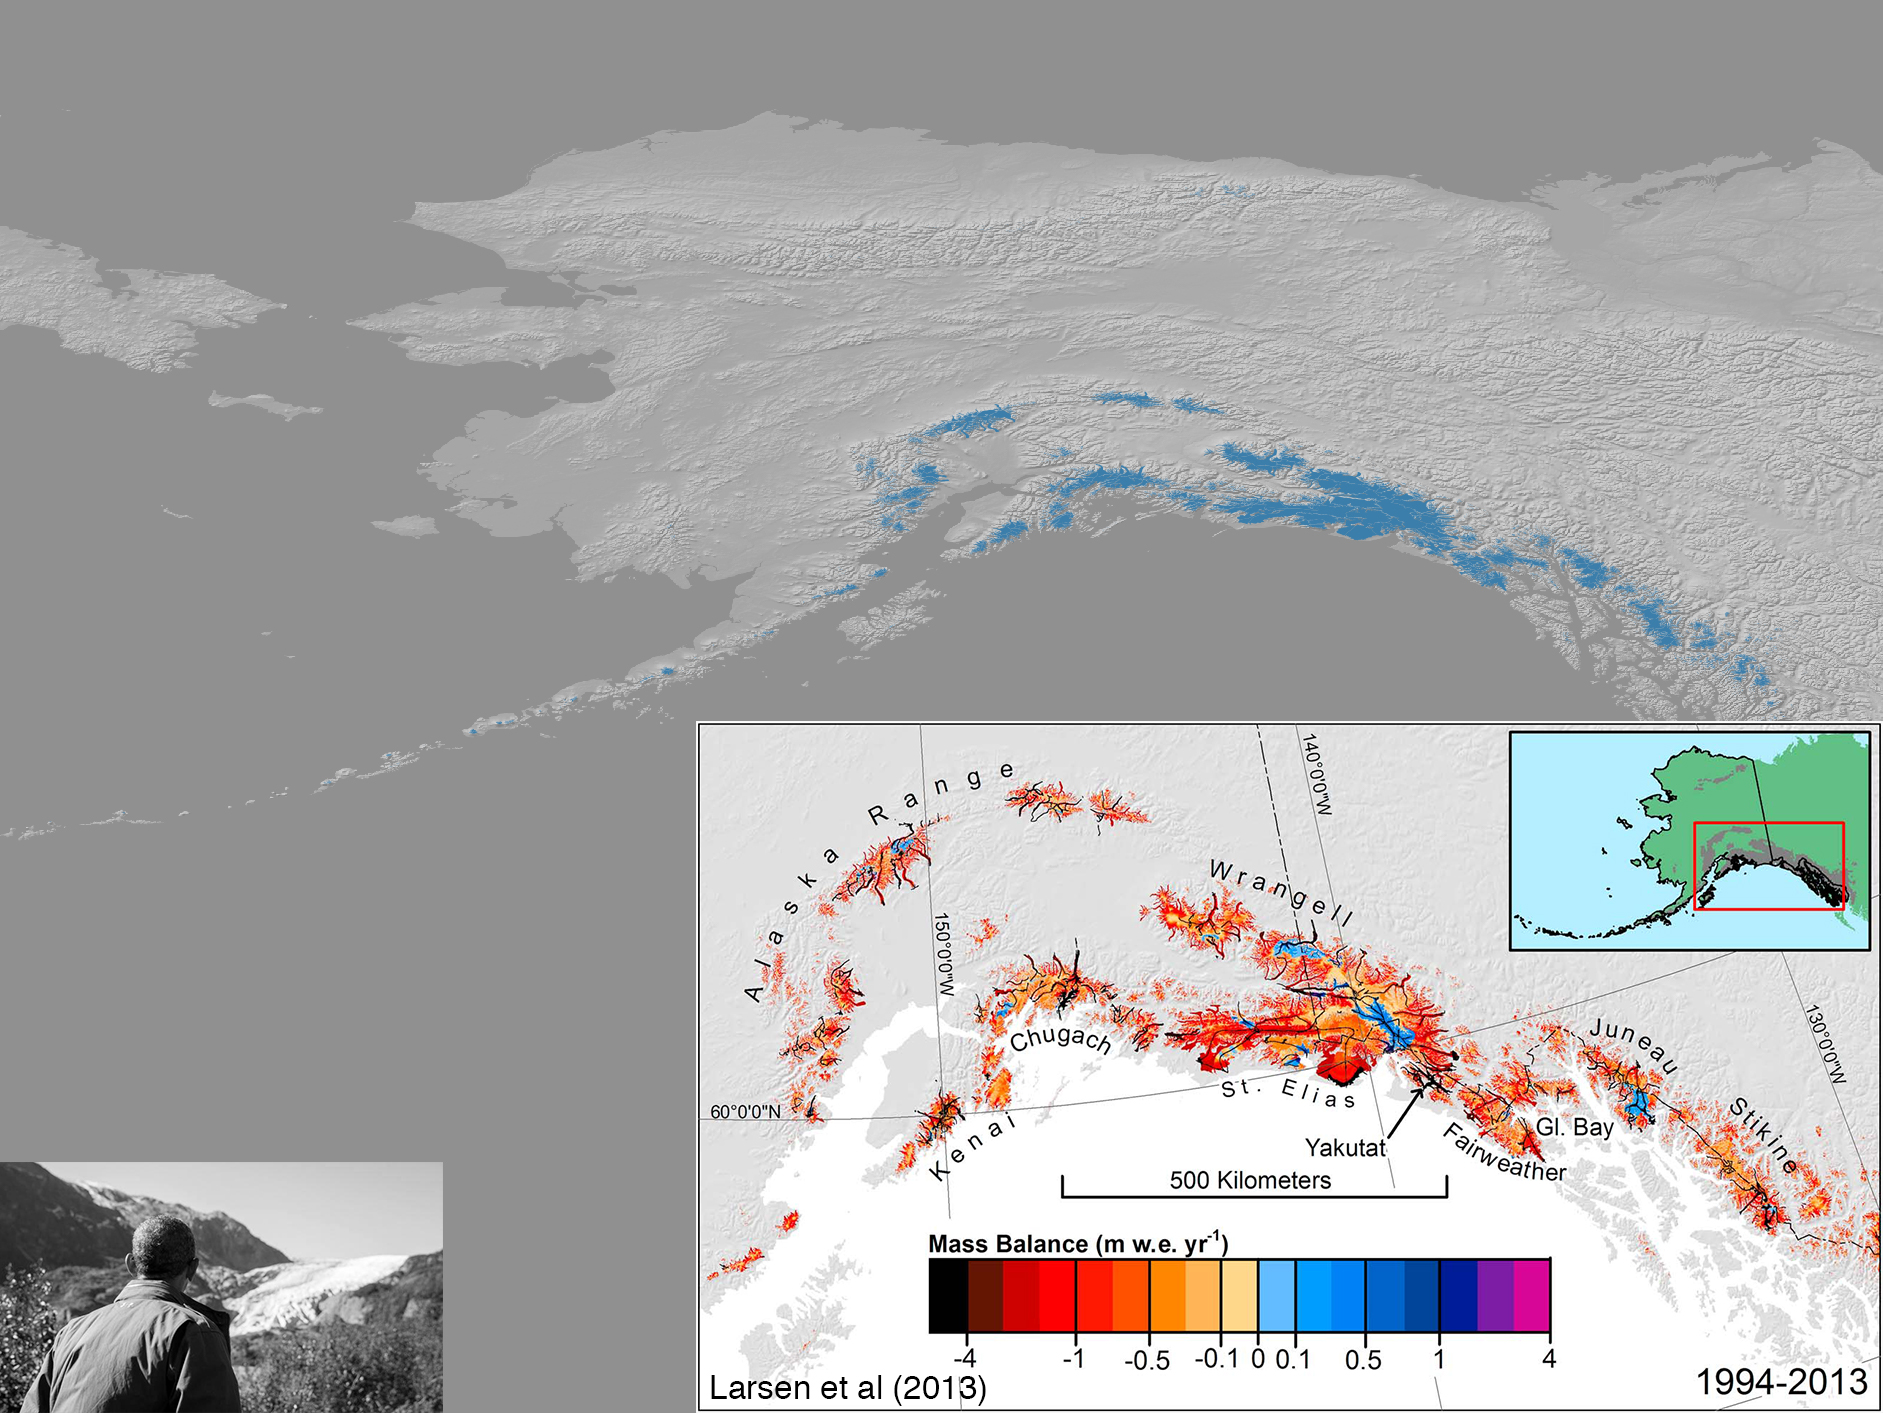
\includegraphics[width=\paperwidth]{ak_glacierized_area_16x12}};}
}



\begin{frame}{Melting Glaciers in Alaska: Columbia Glacier}
  \begin{figure}
   \movie[showcontrols=true,autostart,loop,width=12cm]{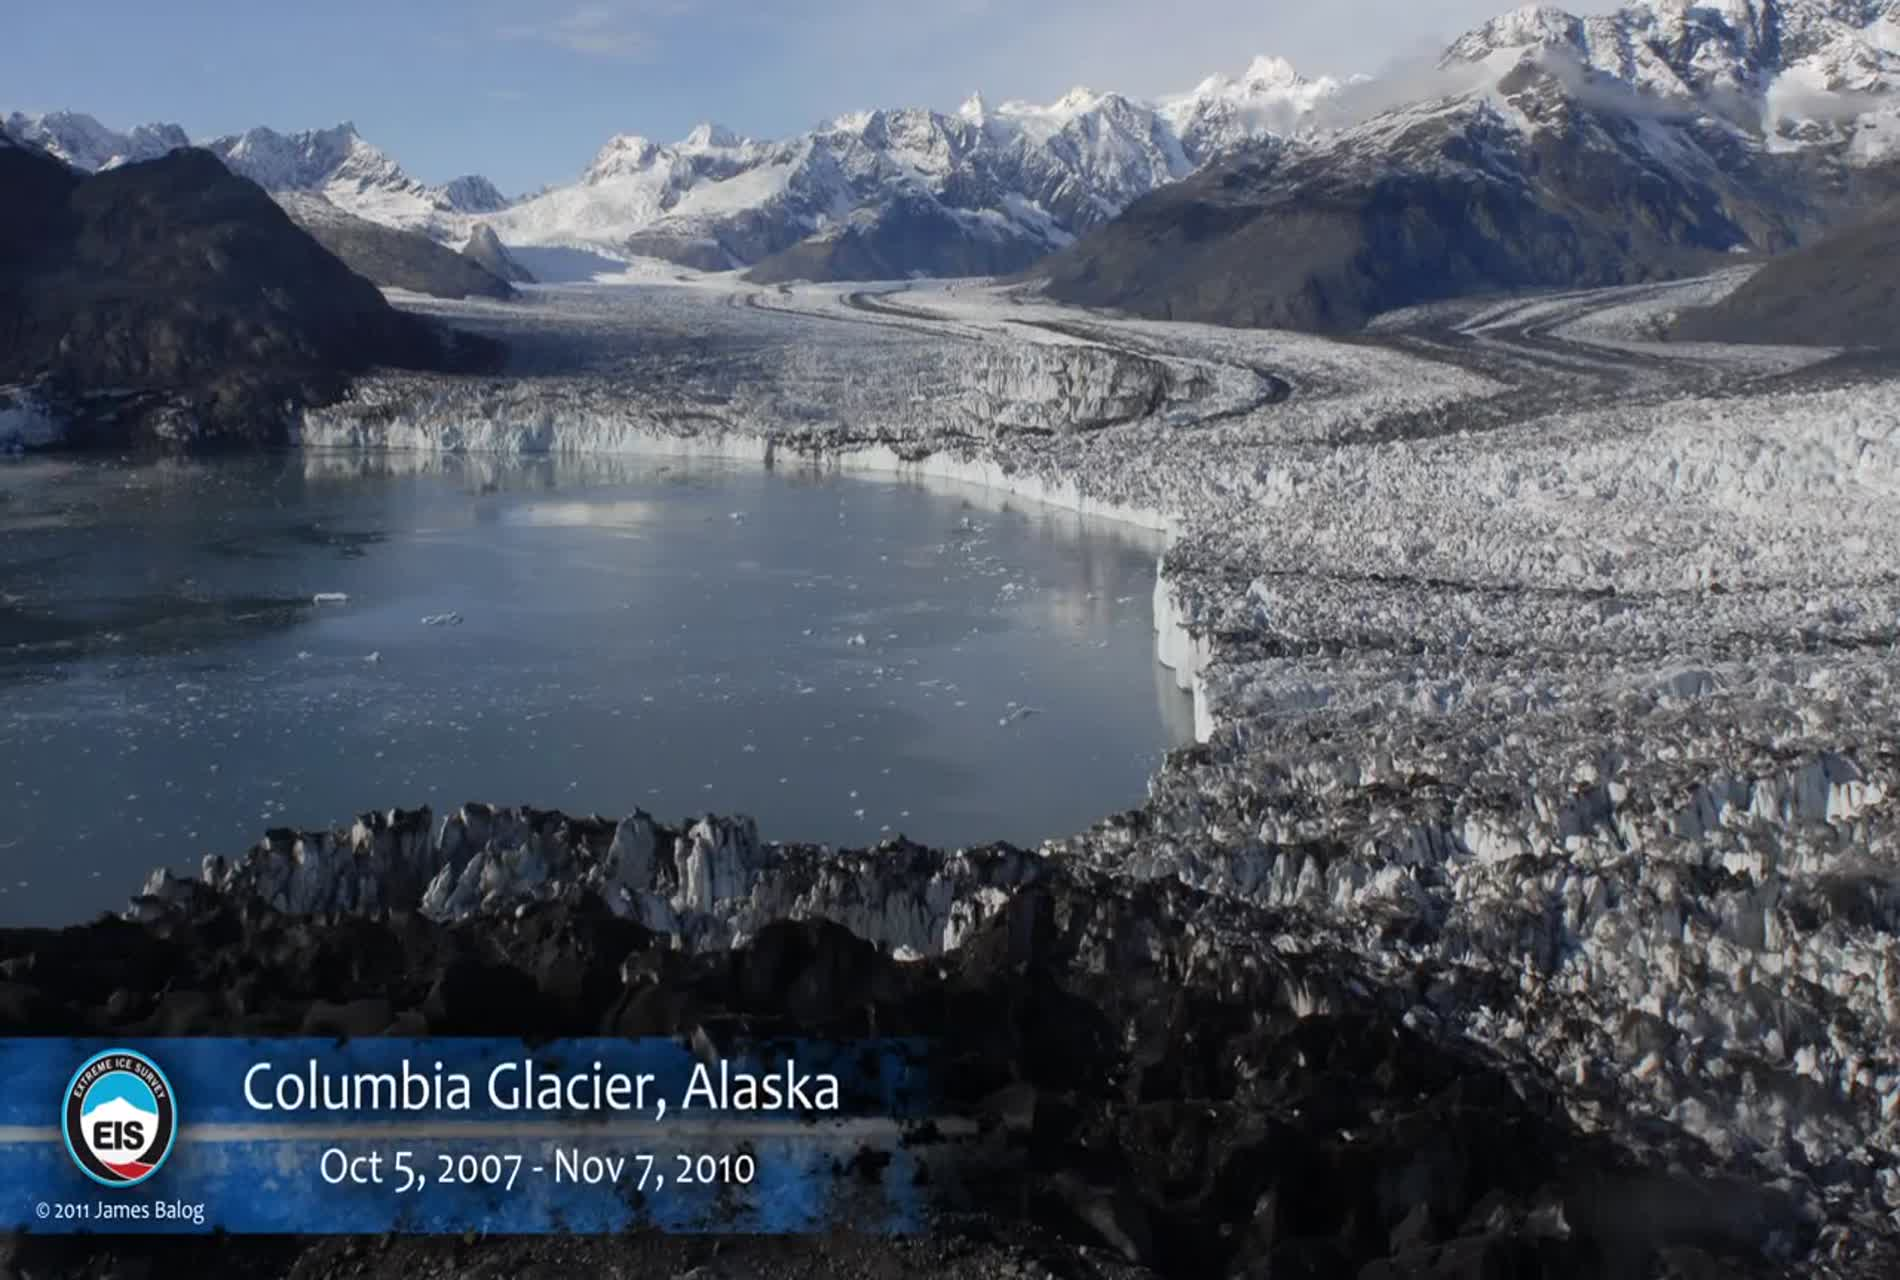
\includegraphics[width=12cm]{columbia-eis}}{columbia-eis.mov}
  \end{figure}
  \note[item]{I was wondering if this happens somewhere else?}
  \note{In Alaska, they are changing too. Columbia glacier for example.}
  \note{Who has been to Columbia Glacier near Valdez?}
  \note{When British explorers first surveyed it in 1794, its front edge (terminus) extended to the northern edge of Heather Island, a small island. The glacier held that position until 1980, when it began a rapid retreat that continues today.}
\end{frame}


% \begin{frame}{Glacier Change in Alaska: Columbia Glacier}
%   \movie[showcontrols=true,autostart,loop,width=12cm]{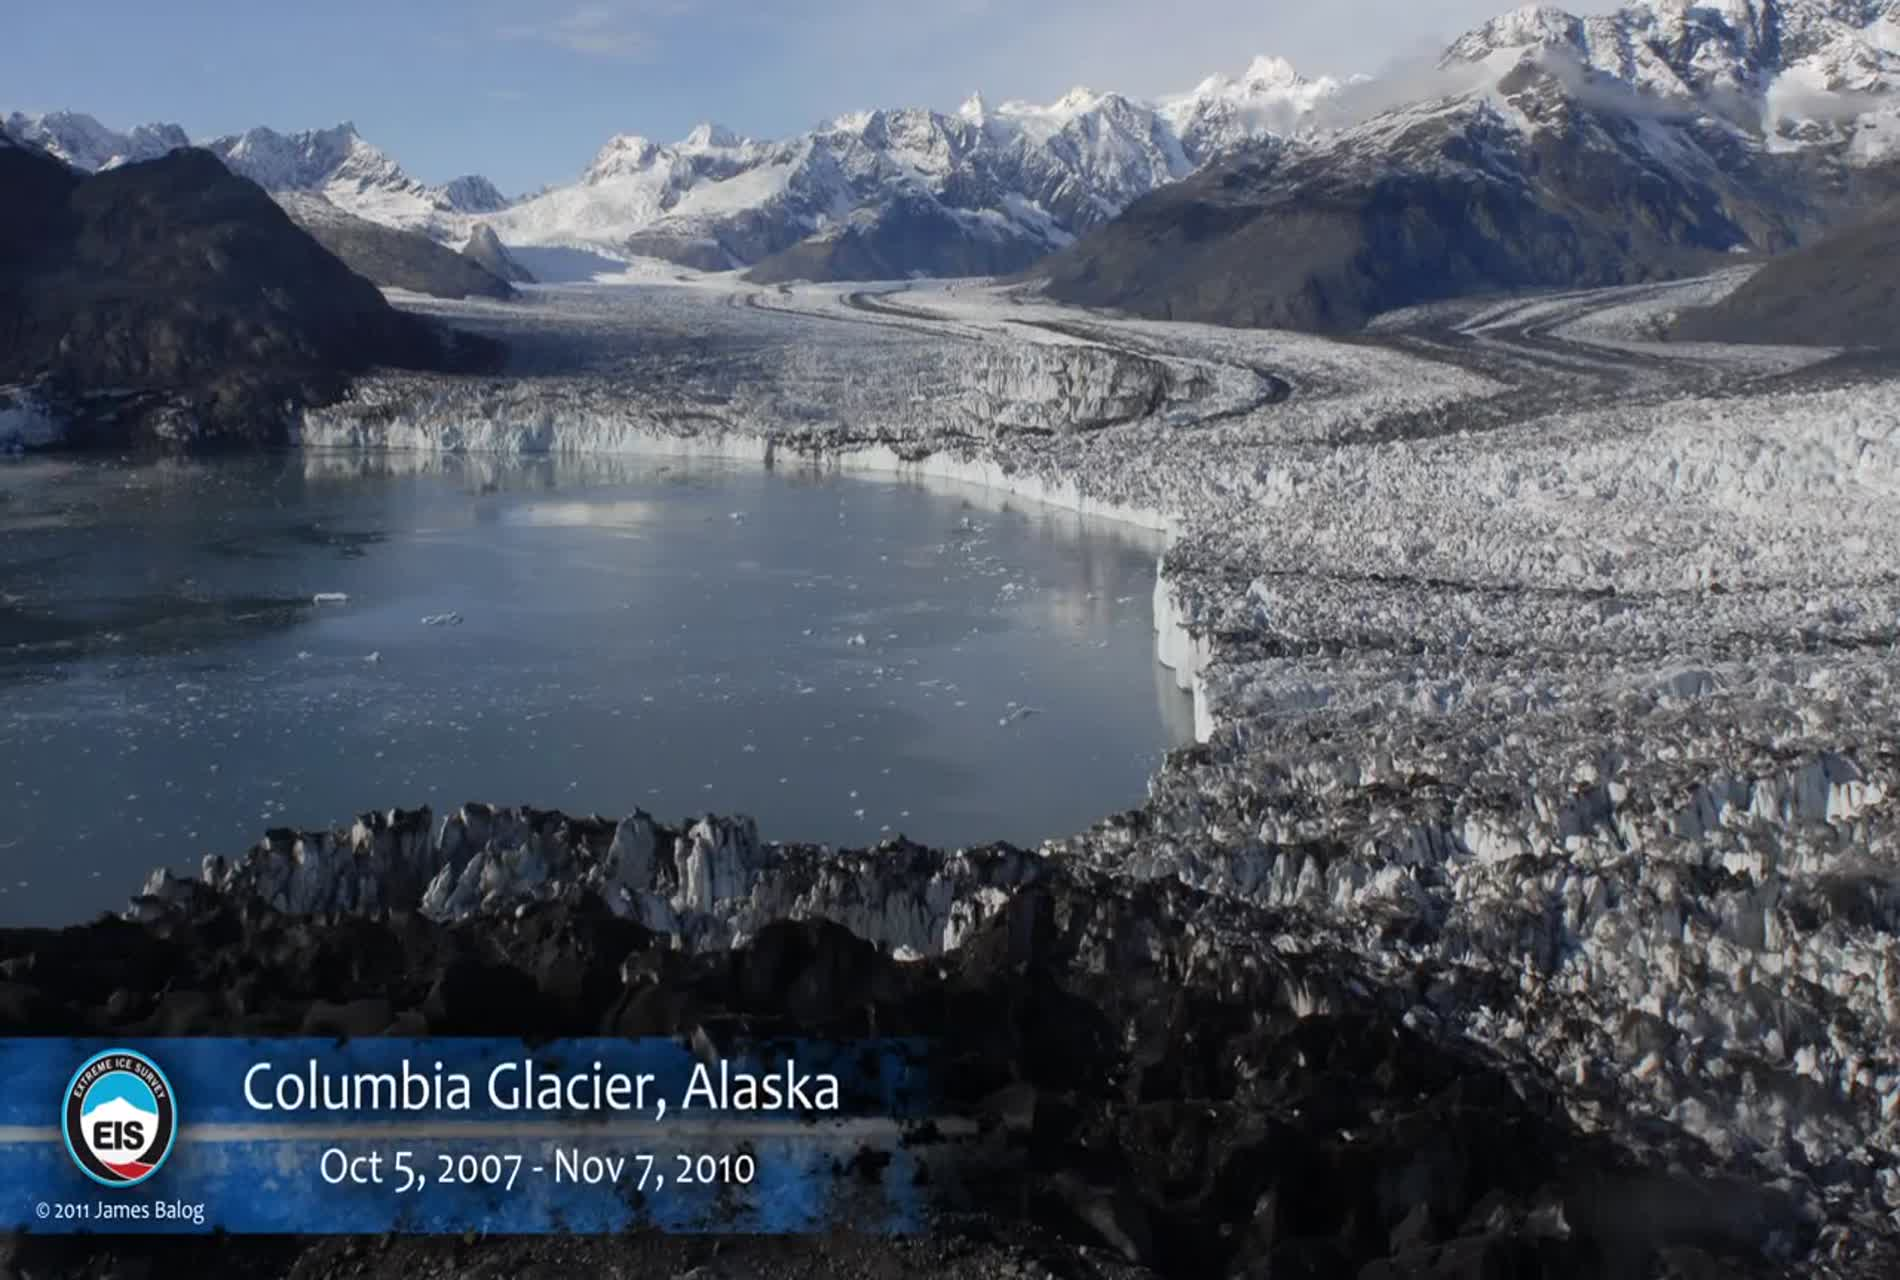
\includegraphics[width=12cm]{columbia-eis}}{columbia-eis.mov}
% \end{frame}


\setbeamertemplate{background canvas}
{
  \tikz{\node[inner sep=0pt,opacity=0.75] {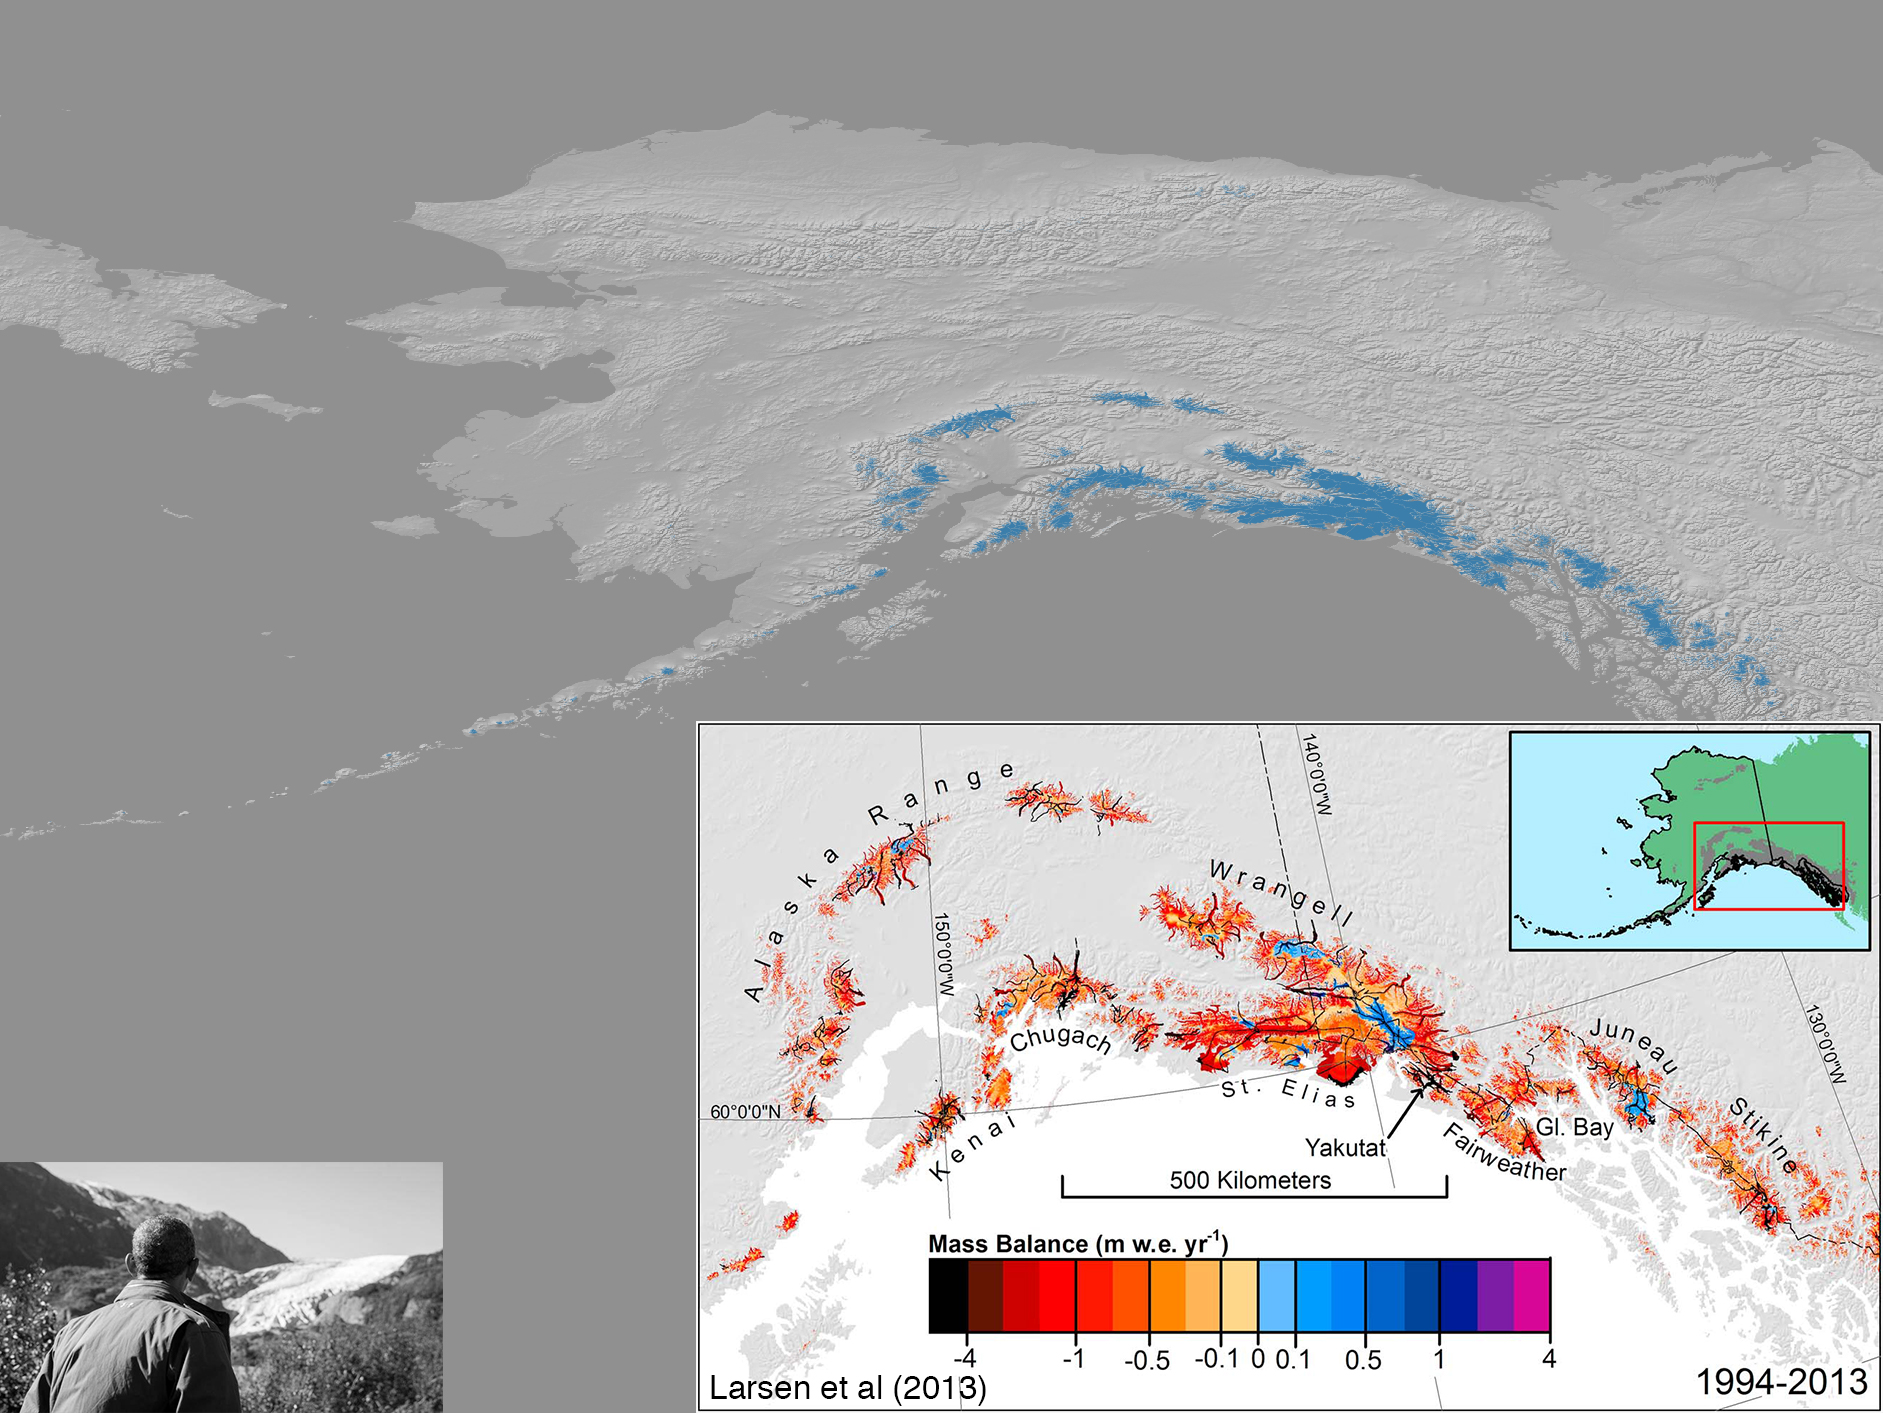
\includegraphics[width=\paperwidth]{ak_glacierized_area_melt_16x12}};}
}

\begin{frame}{Melting Glaciers in Alaska}
  \begin{itemize}
  \item total mass loss 1994--2013 from AK glaciers: 75$\pm$11 Gt/yr loss $\Rightarrow$ 5\,cm (2\,in) layer of water covering Alaska
  \end{itemize}
  \note[item]{Explain thinning and mass loss}
  \note[item]{Columbia Glacier is not alone}
  \note[item]{As recent study by UAF's Chris Larsen and others shows that many glaciers are melting}
  \note[item]{The red colors indicate glaciers that have lost mass between 1994 and 2013}
  \note[item]{while blue color indicate mass gain}
  \note[item]{there are many more glaciers losing mass than gaining mass}
  \note[item]{Between 94 and 2013, Alaskan glaciers lost a combined 75 Gt per year}
  \note[item]{How much are 75 giga ton?}
  \note[item]{If you spread 75 Gt of water evenly over Alaska}
  \note[item]{and here we assume Alaska is flat}
  \note[item]{we would stand in 5cm deep water}

\end{frame}

\setbeamertemplate{background canvas}
{
}


% \setbeamertemplate{background canvas}
% {
%   \tikz{\node[inner sep=0pt,opacity=0.75] {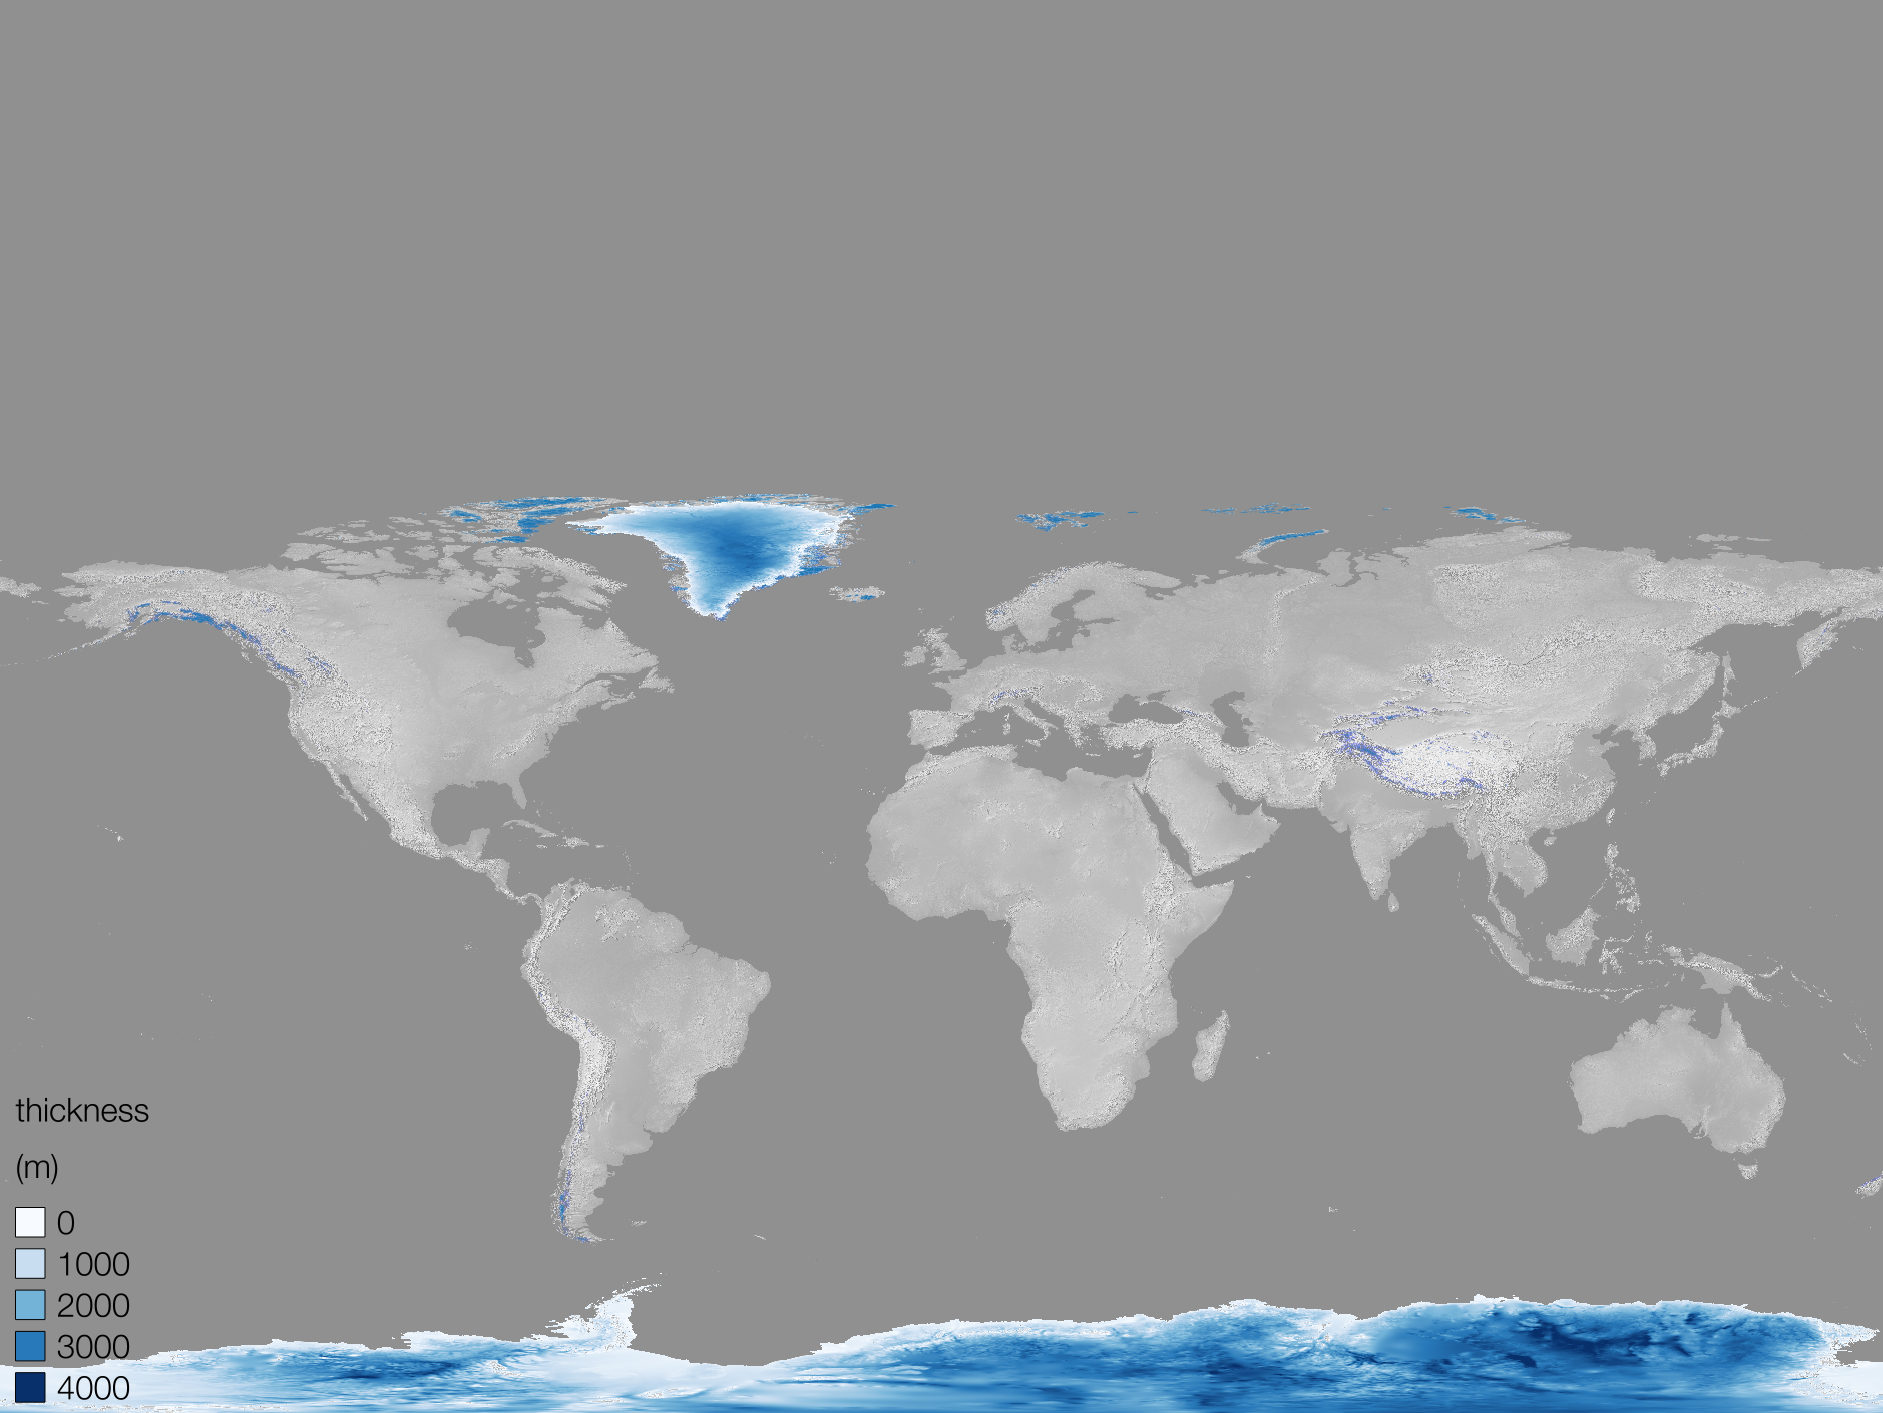
\includegraphics[width=\paperwidth]{world_glacierized_area_16x12}};}
% }

% \begin{frame}{Glacier Change Worldwide}
%   \begin{itemize}
%     \item Presently, 10\,\% of land area is covered with ice
%     \item That's about 10 times the size of Alaska
%   \end{itemize}
% \end{frame}


% \setbeamertemplate{background canvas}
% {
% }

\begin{frame}{Melting Glaciers Everywhere: The Biggest Losers}
  \begin{figure}
    {Alaska \qquad---\qquad West Greenland \qquad---\qquad West Antartica}
    \\[1em]
    \includegraphics<1>[width=1\textwidth]{grace-world-2003-2010-01}
  \end{figure}
  \note[item]{But maybe Switzerland and Alaska are the exception?}
  \note[item]{Glaciers are melting worldwide}
  \note[item]{This figure shows glacier mass loss world wide}
  \note[item]{Again, red colors indicate mass loss}
  \note[item]{The biggest red areas are Alaska, Greenland, and West Antartica}
  \note[item]{These are the biggest losers}
\end{frame}

\setbeamertemplate{background canvas}
{
  \tikz{\node[inner sep=0pt,opacity=.6] {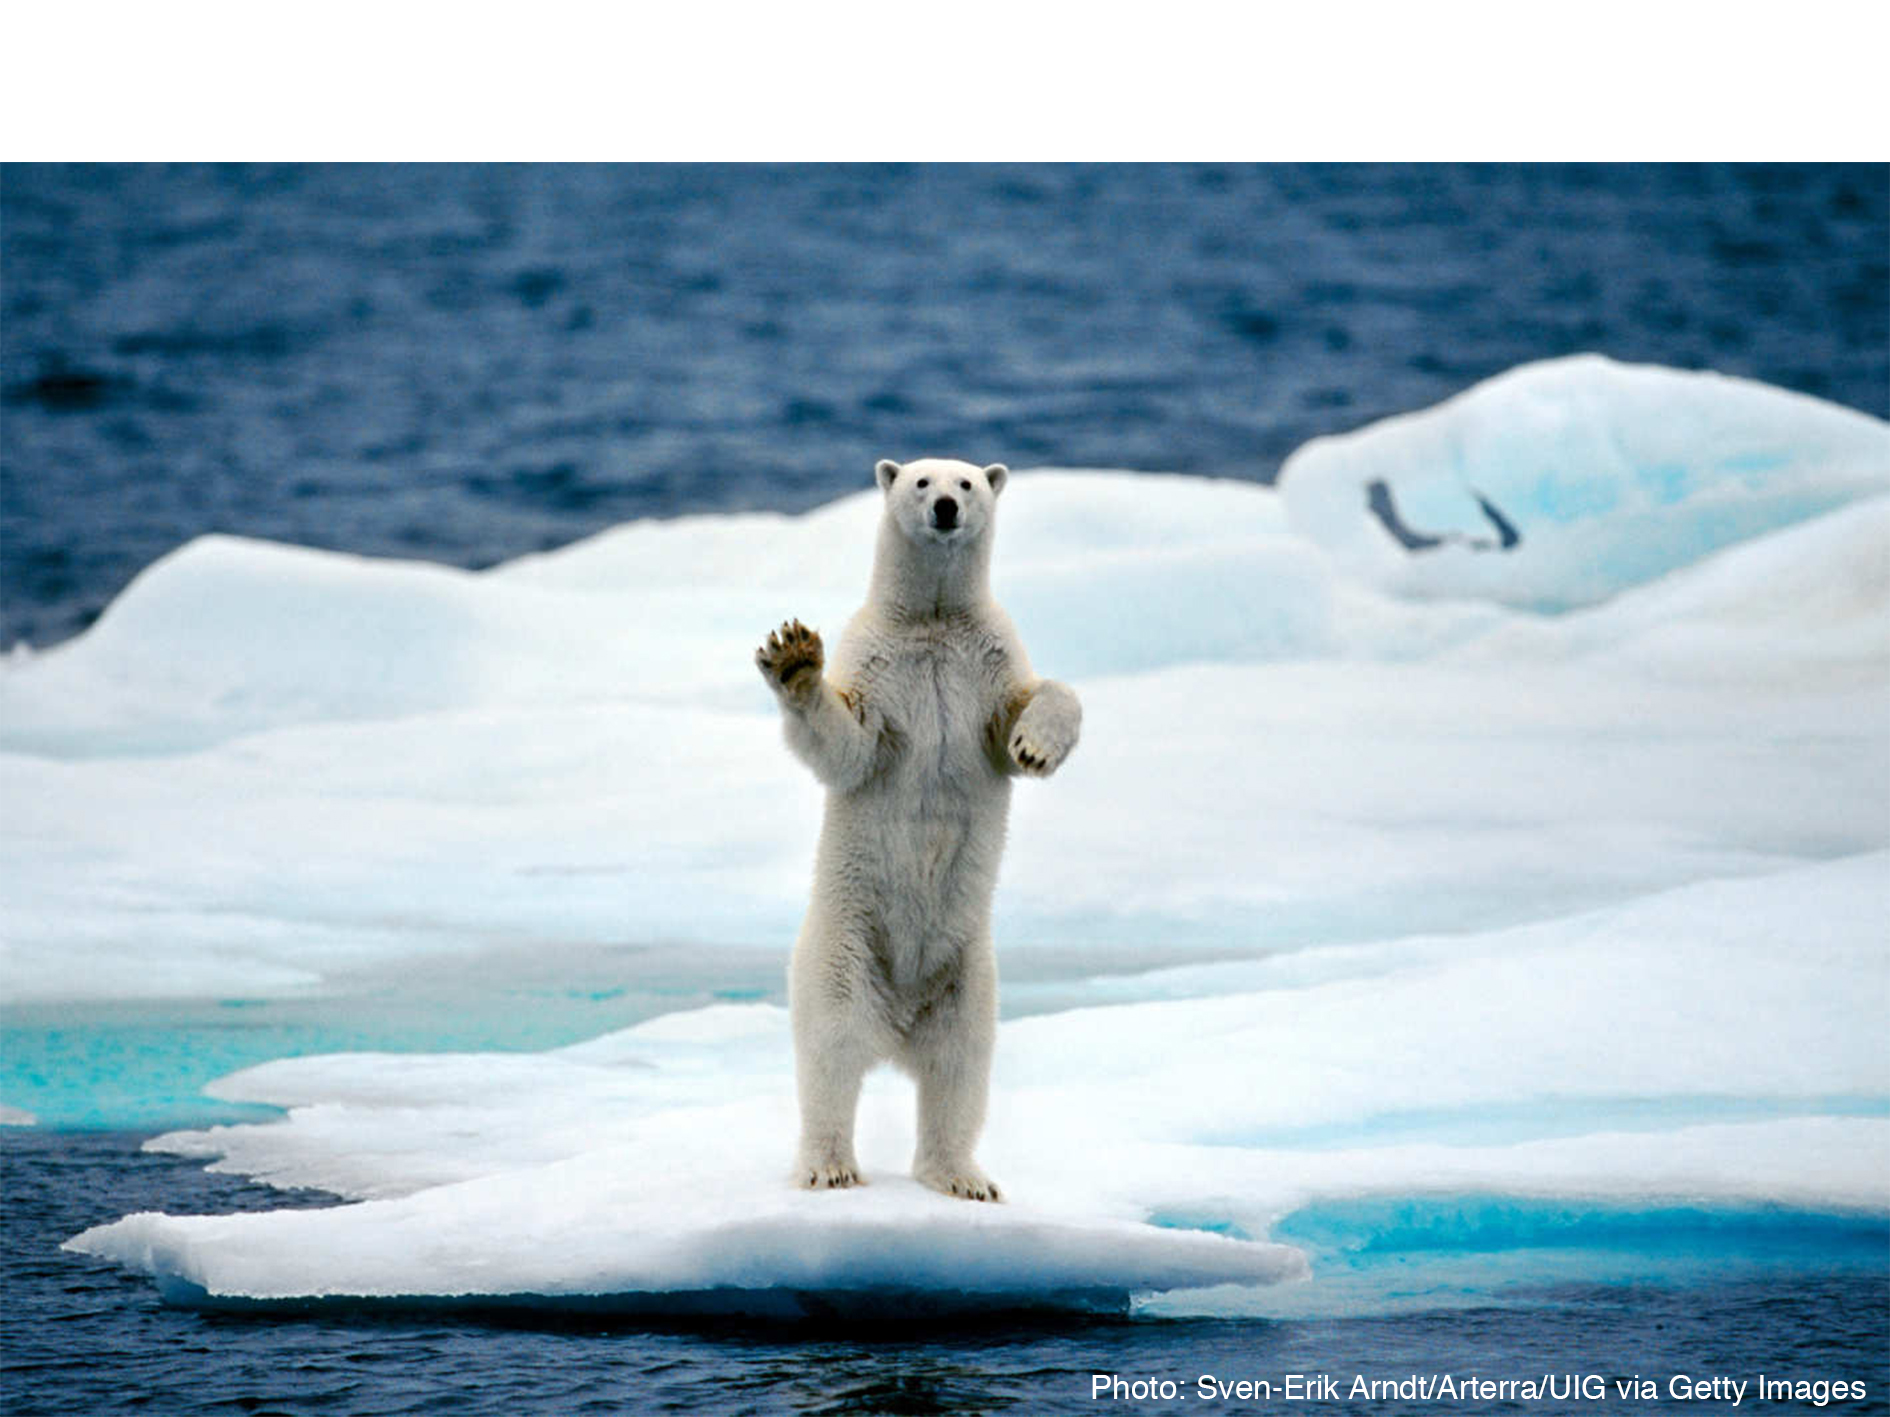
\includegraphics[height=\paperheight,width=\paperwidth]{polar-bear-wcredit}};}
}


\begin{frame}{}
  \centering{``Hasn't the Climate Changed Before?''}
  \note[item]{But wait}
  \note[item]{aren't glaciers and the climate constantly changing}
  \note[item]{number one question}
  \note[item]{seat neighbor in airplane}
\end{frame}

\setbeamertemplate{background canvas}
{
}


\begin{frame}{Glacials and Interglacials}
  \begin{columns}[c]
    \begin{column}{.45\linewidth}
      \begin{figure}
        \includegraphics<1>[height=7.5cm]{ice-age-movie-1}
        {\\ \alert{glacial}}
      \end{figure}
    \end{column}
    \begin{column}{.45\linewidth}
      \begin{figure}
        \includegraphics<1>[height=7.5cm]{ice-age-movie-meltdown}
        {\\ \alert{interglacial}}
      \end{figure}
    \end{column}
  \end{columns}
  \note[item]{As we learned from Hollywood}
  \note[item]{there have been Ice Ages and Meltdowns}
  \note[item]{or as we call it: glacials and interglacials}
  \note[item]{Visualize warm / cold}
\end{frame}

\setbeamertemplate{background canvas}
{
  \tikz{\node[inner sep=0pt,opacity=1] {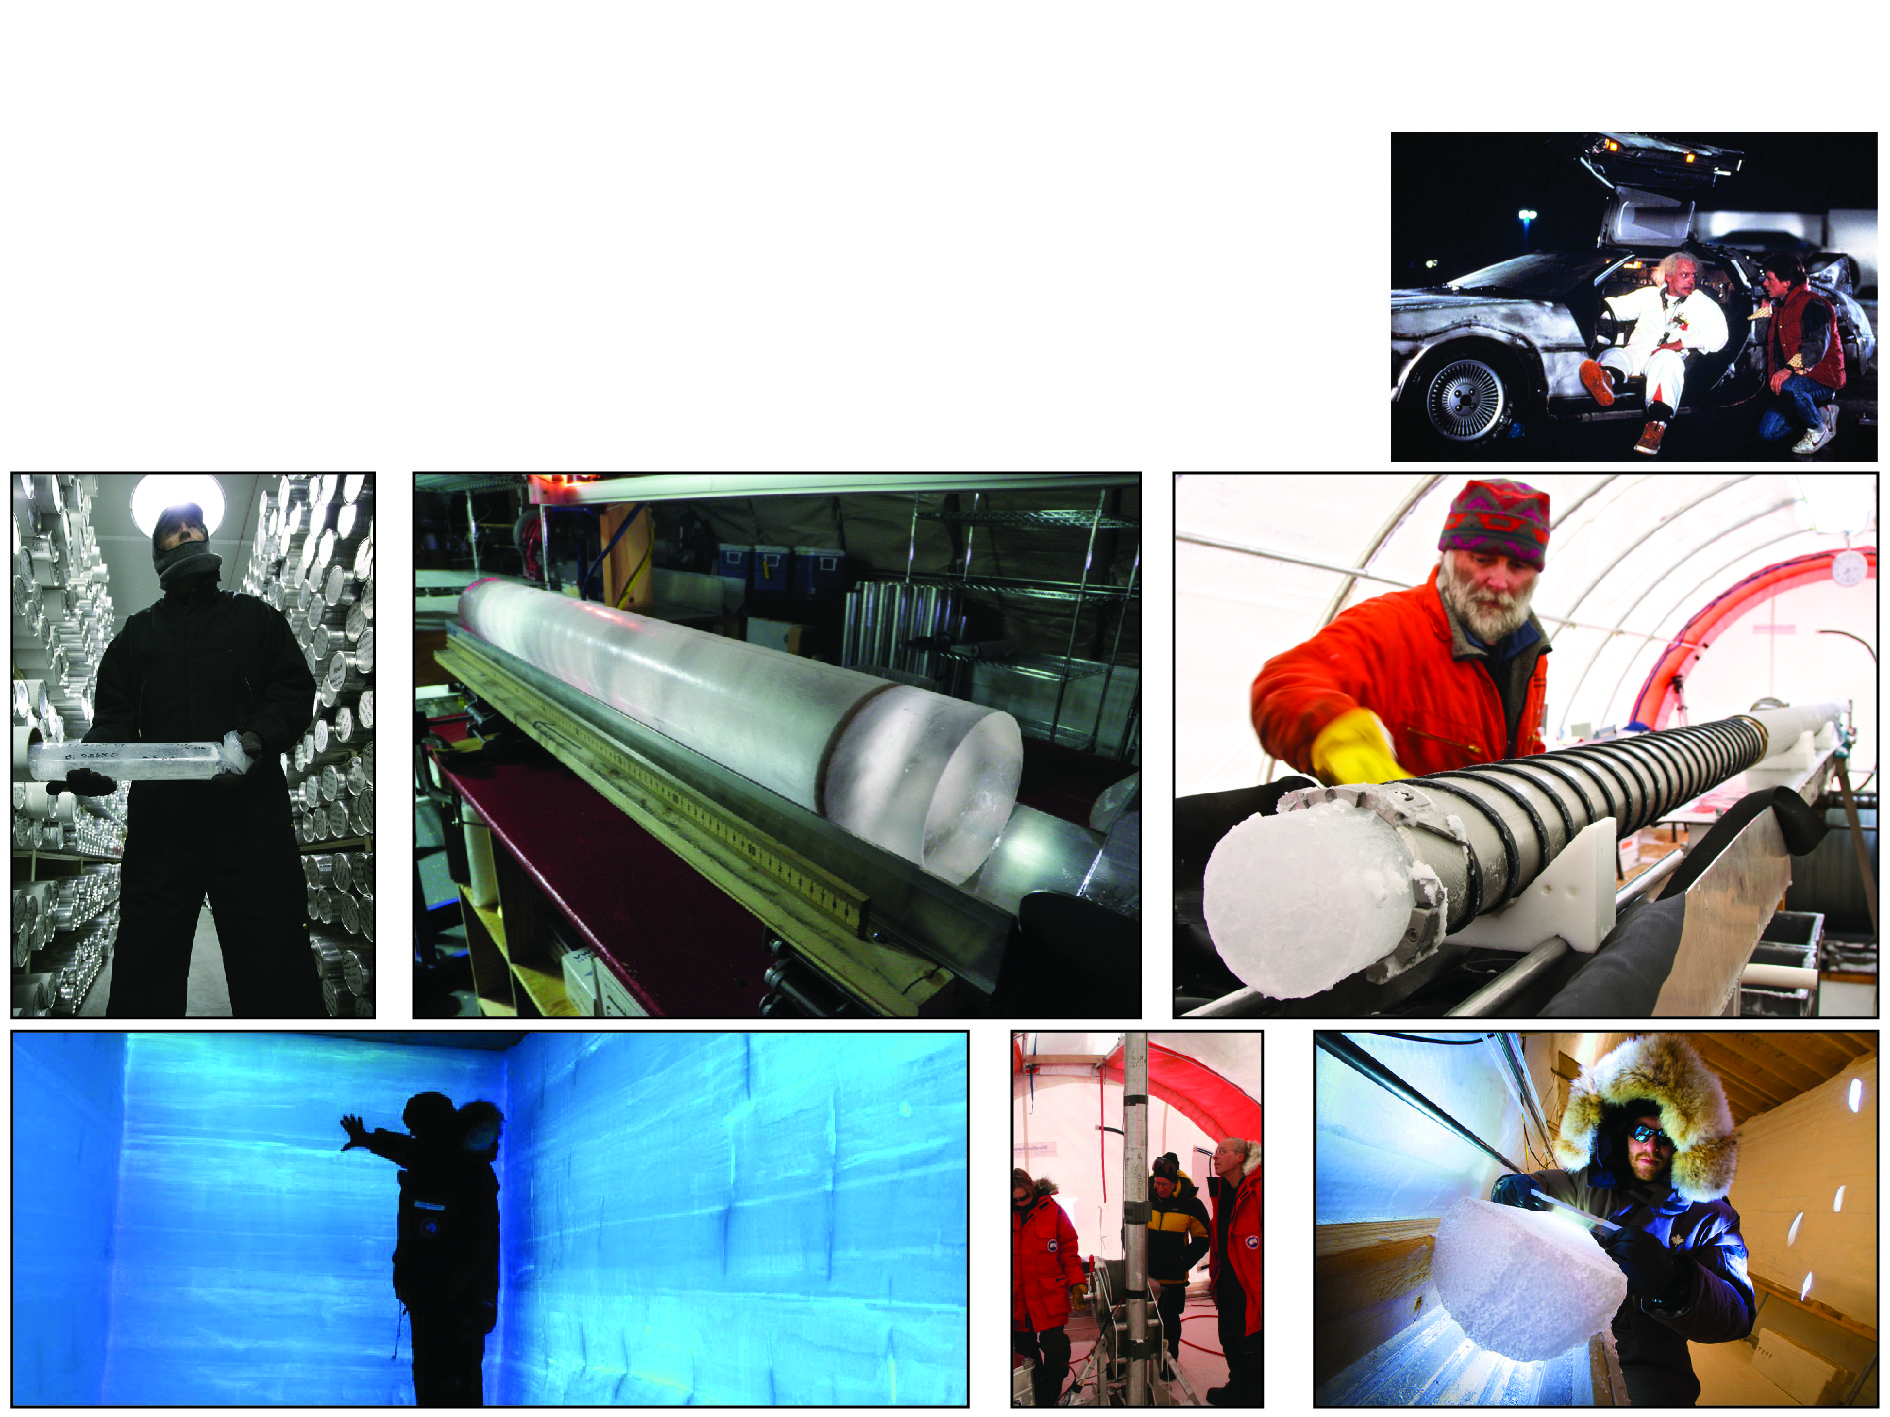
\includegraphics[height=\paperheight,width=\paperwidth]{ice-core-collage}};}
}

\begin{frame}{Ice Cores: The 2-mile Time Machine}
  \note[item]{We know about glacials and interglacials from}
  \note[item]{geologic evidence and from ice cores}
  \note[item]{Why do is core works, what does it represent, snow turns into ice, each layer is a time capsule}
  \note[item]{An ice cores are like a big archive that}
  \note[item]{stores information about past climate}
  \note[item]{The information is locked up in tiny little air bubbles trapped within the ice}
  \note[item]{Ice cores from Greenland and Antartica are up to 2 mile deep}
  \note[item]{the deeper you go, the older the ice gets}
  \note[item]{It's like a time capsule, a two mile long time machine}
  \note[item]{climate scientists have analyzed ice that is up to 800,000 years old}
  \note[item]{This gives us a pretty good picture about climate varibility over almost a million years}
\end{frame}

\setbeamertemplate{background canvas}
{
  \tikz{\node[inner sep=0pt,opacity=0.4] {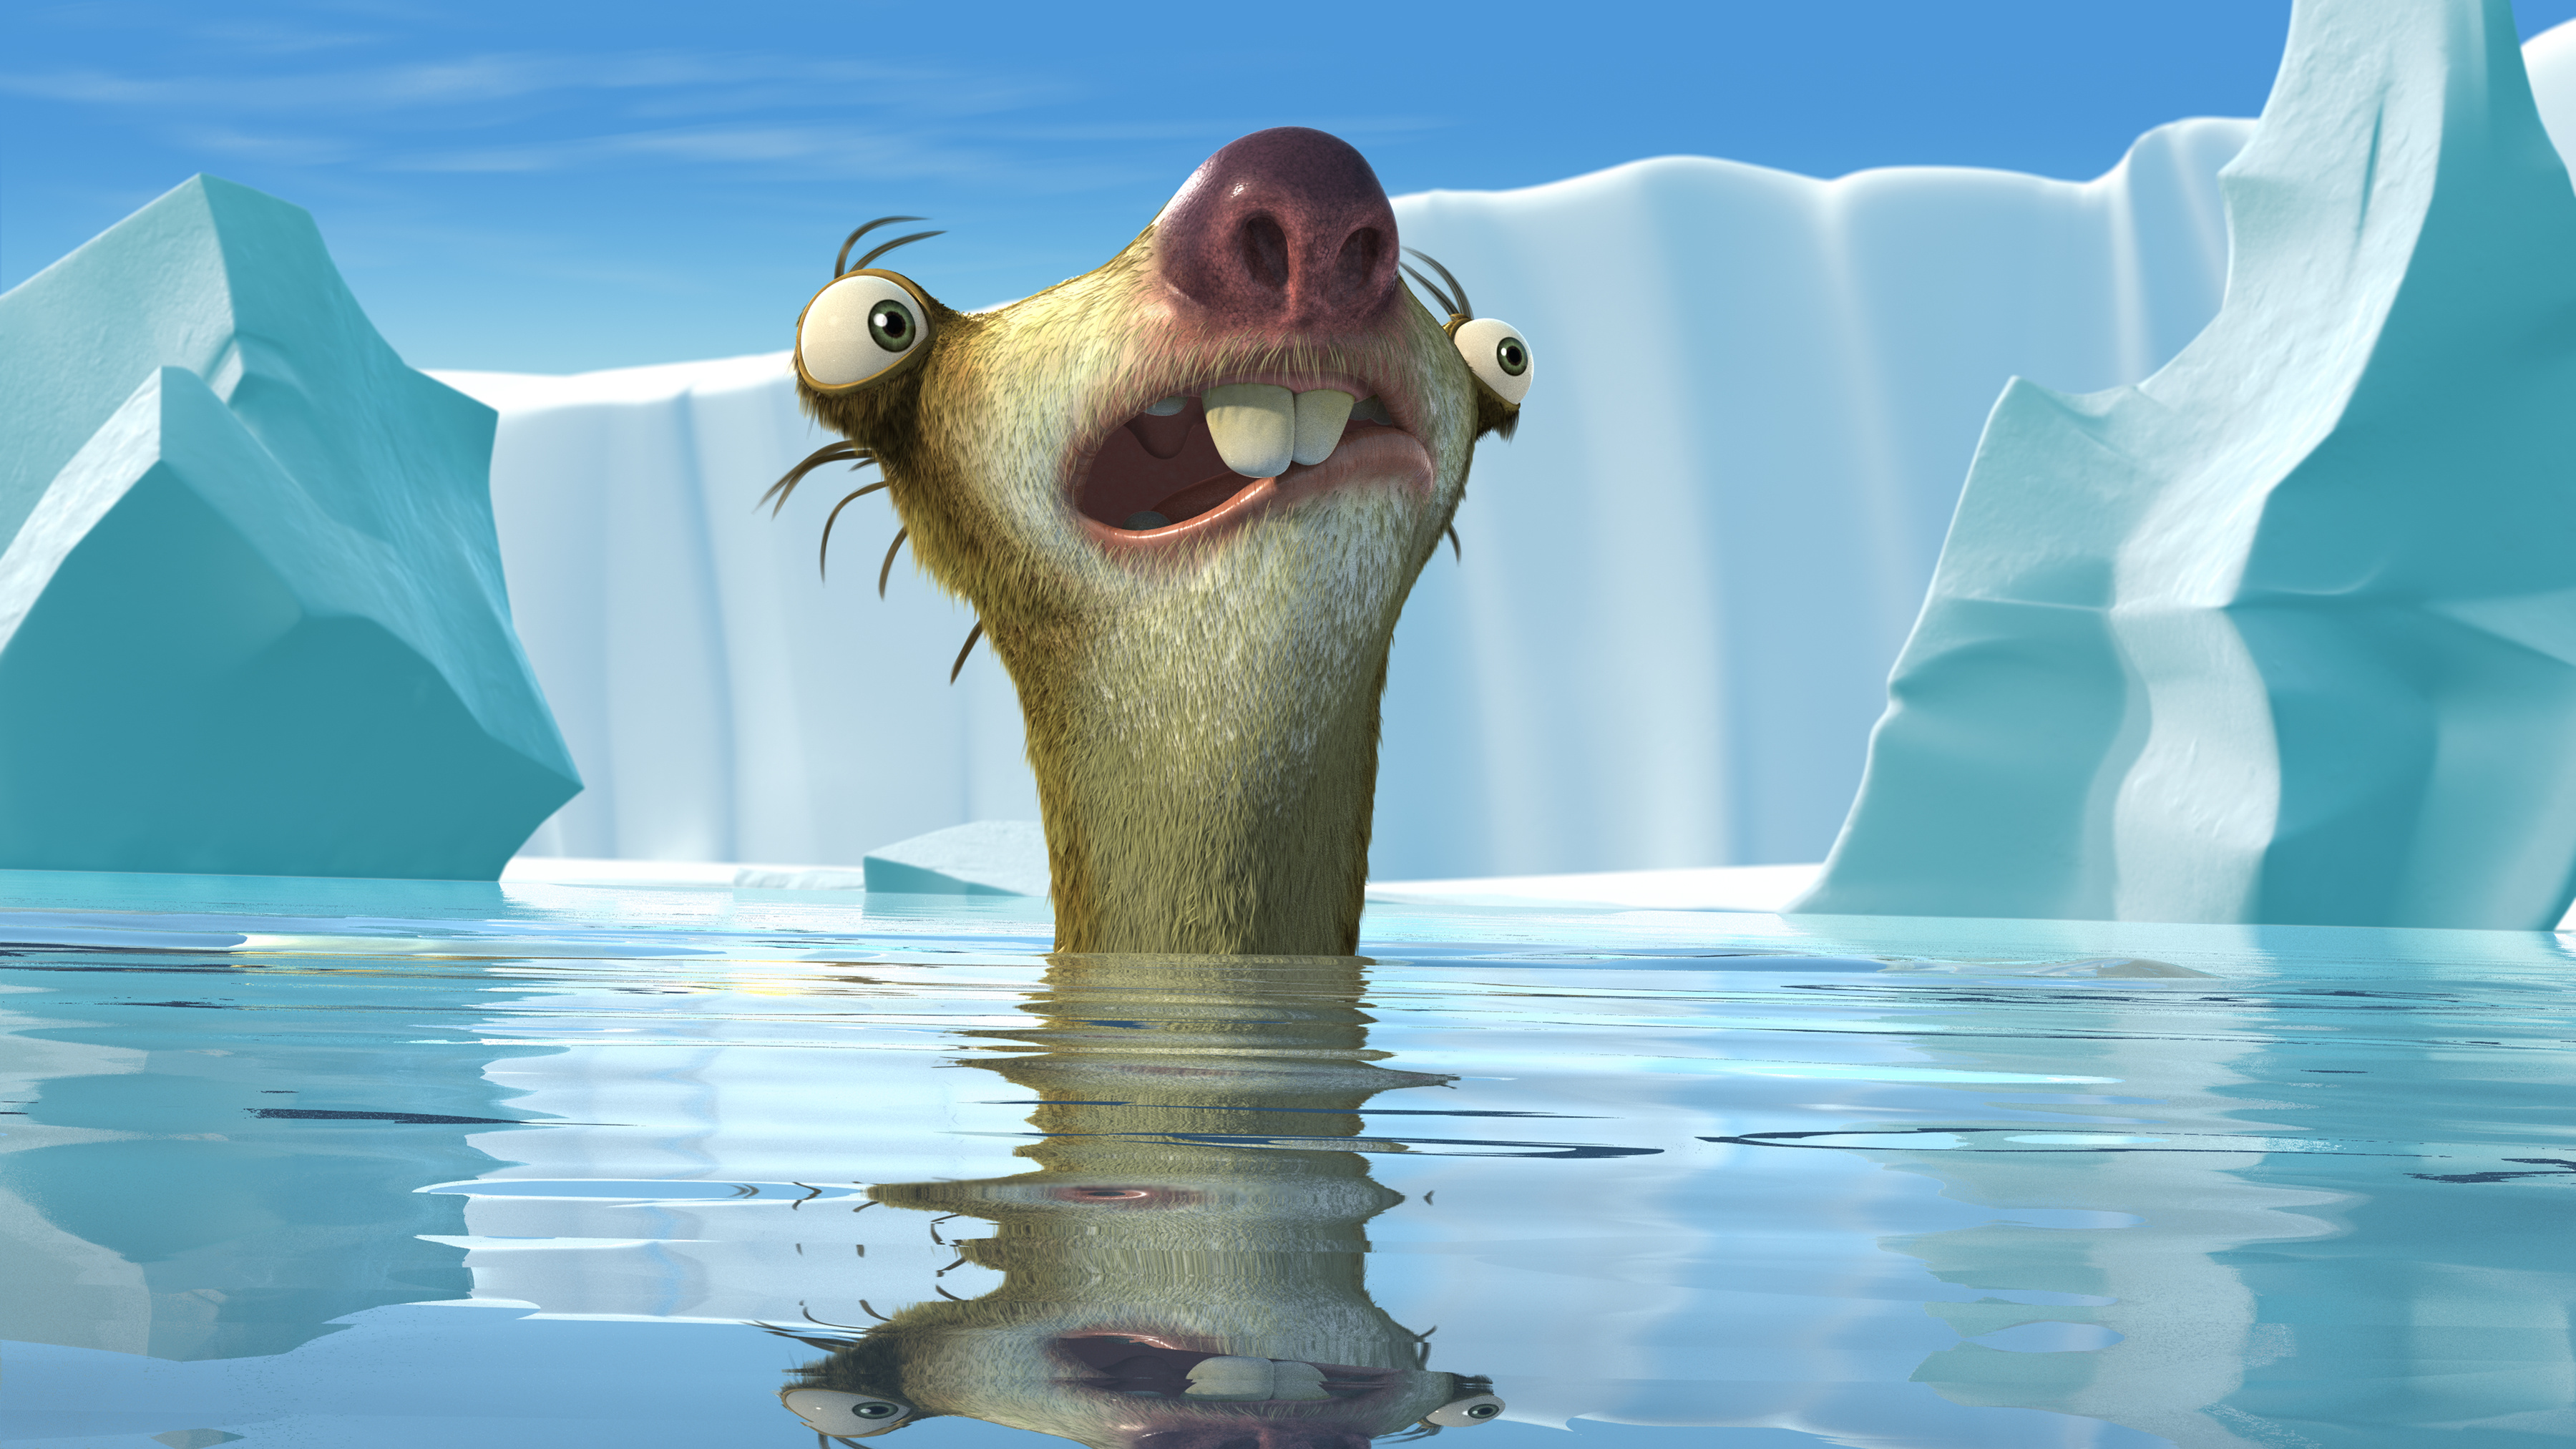
\includegraphics[height=\paperheight,width=\paperwidth]{ice-age}};}
}

\begin{frame}{Climate History}
  \vspace{.15cm}
  \begin{figure}
    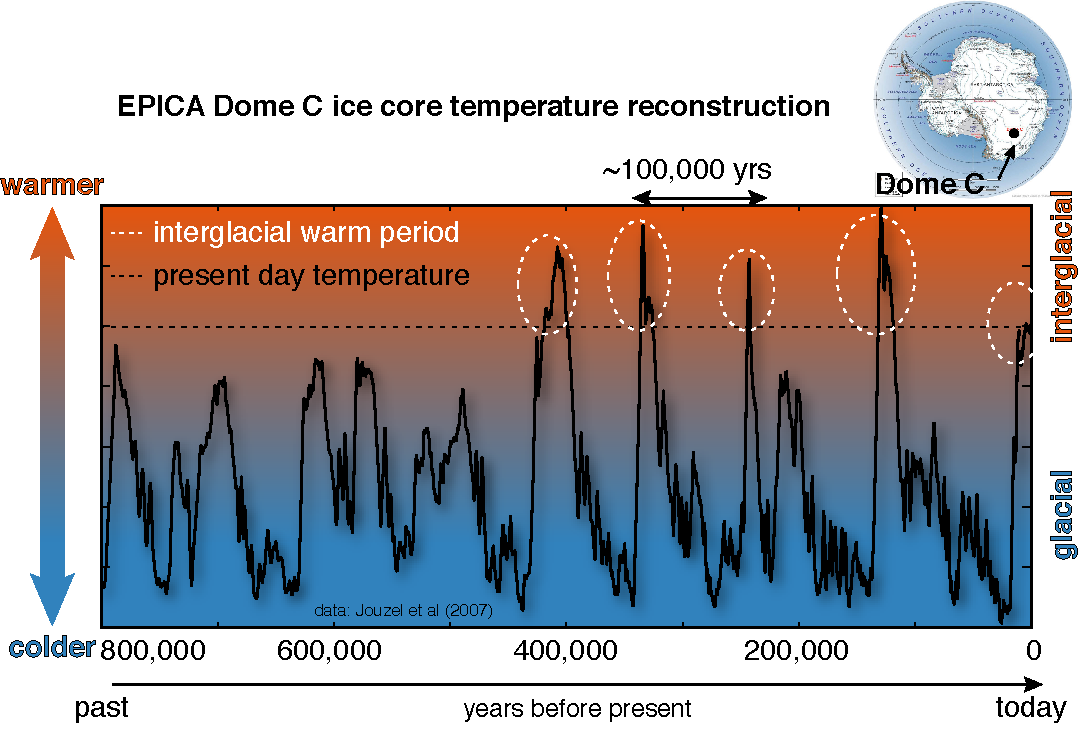
\includegraphics[width=\textwidth]{epica-temp}
  \end{figure}
  \note[item]{Flip time axis}
  \note[item]{Let's look at temperature changes}
  \note[item]{What is this, explain time axis}
  \note[item]{We see that most of the time, it was cold and we were in an Ice Age}
  \note[item]{But find 5 distinct warm periods during the past half a million years, about 100,000 years apart}
  \note[item]{and we are currently in the fifth warm period or interglacial that started about 12,000yrs ago}
  \note[item]{There have been times when it was warmer than today}
  \note[item]{but the last time it was warmer was more the 100,000yrs ago }
  \note[item]{This cycle of glacials and interglacials is driven by how much sun light the Northern Hemisphere receives}
  \note[item]{The physics behind this is well understood but would take up a whole other talk}
\end{frame}


\begin{frame}{So what makes the past 100\,yrs so special}
  \vspace{.15cm}
  \begin{figure}
    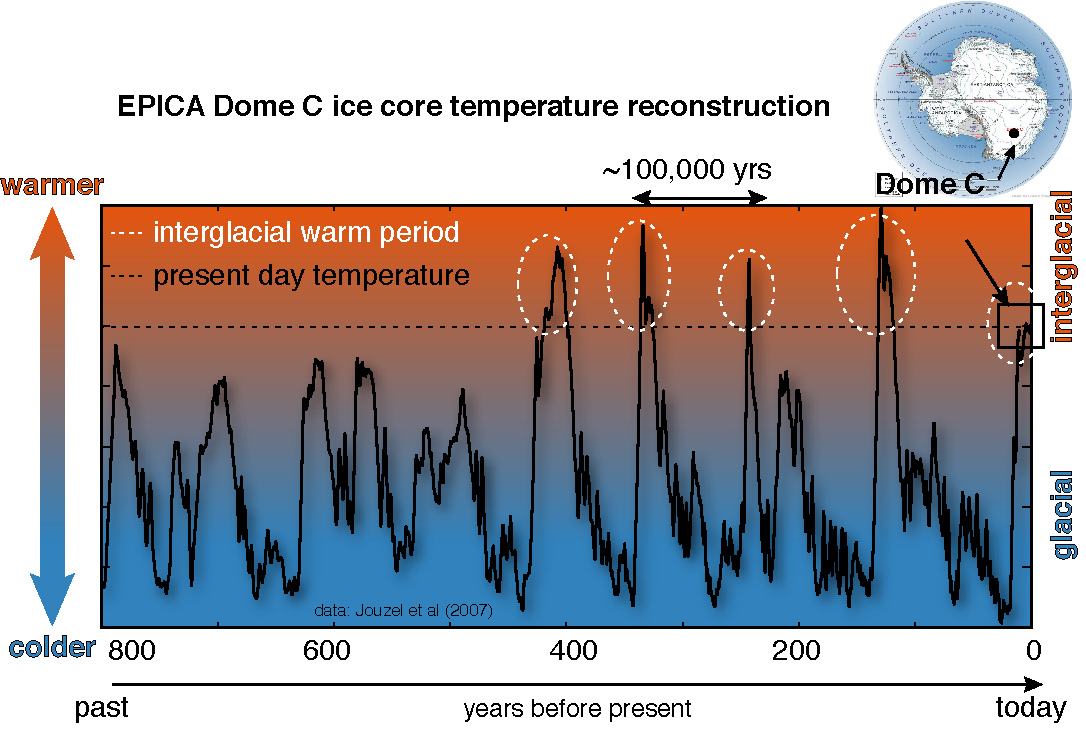
\includegraphics[width=\textwidth]{epica-temp-box}
  \end{figure}
  \note[item]{We hear about all the crazy stuff going on today, so let's zoom in to present-day}
  \note[item]{So what makes the past 100\,yrs so special}
\end{frame}


\setbeamertemplate{background canvas}
{
}

\begin{frame}{So what makes the past 100\,yrs so special}
  \begin{figure}
    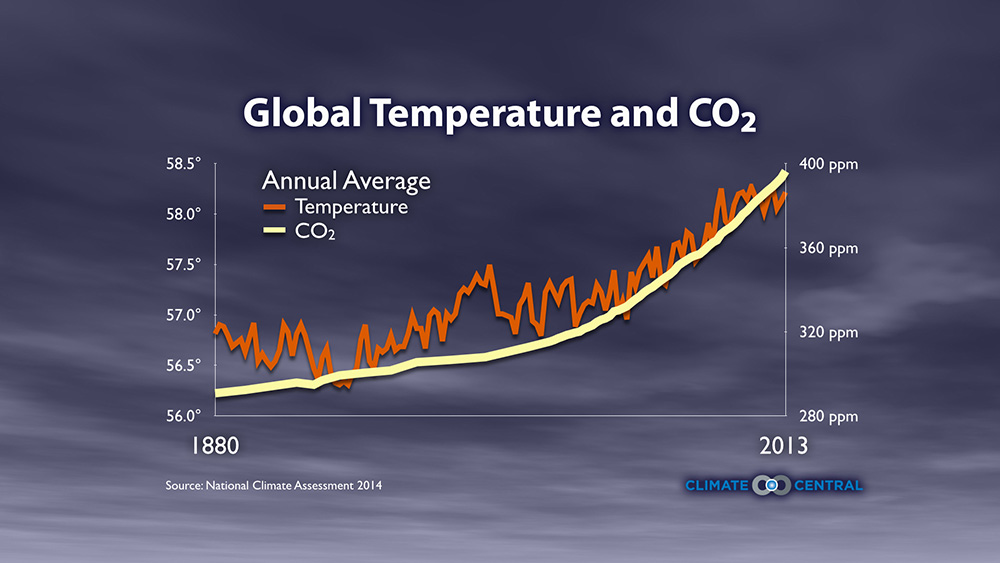
\includegraphics[width=\textwidth]{Global_Temp_and_CO2}
  \end{figure}
  \note[item]{Explain CO2}
  \note[item]{Since I explained a few slides ago that whether we are in}
  \note[item]{an Ice Age or a warm period depends on how much sun we are receiving}
  \note[item]{one could suggest that the sun that is driving the 20th century temperture increase}
  \note[item]{But if we look at sun activity, the sun hasn't been doing much}
  \note[item]{To the contary, sun activity was higher in the fifties and the sixties than today}
  \note[item]{On the other hand, carbon dioxide, shown here with the blue line, has been increasing since the industrial revolution}
  \note[item]{That there is a connection between rising CO2 levels and temperature isn't rocket science}
  \note[item]{in fact the basics have been known since the times of the Civil War}
\end{frame}

  

\setbeamertemplate{background canvas}
  {
     \tikz{\node[inner sep=0pt,opacity=0.5] {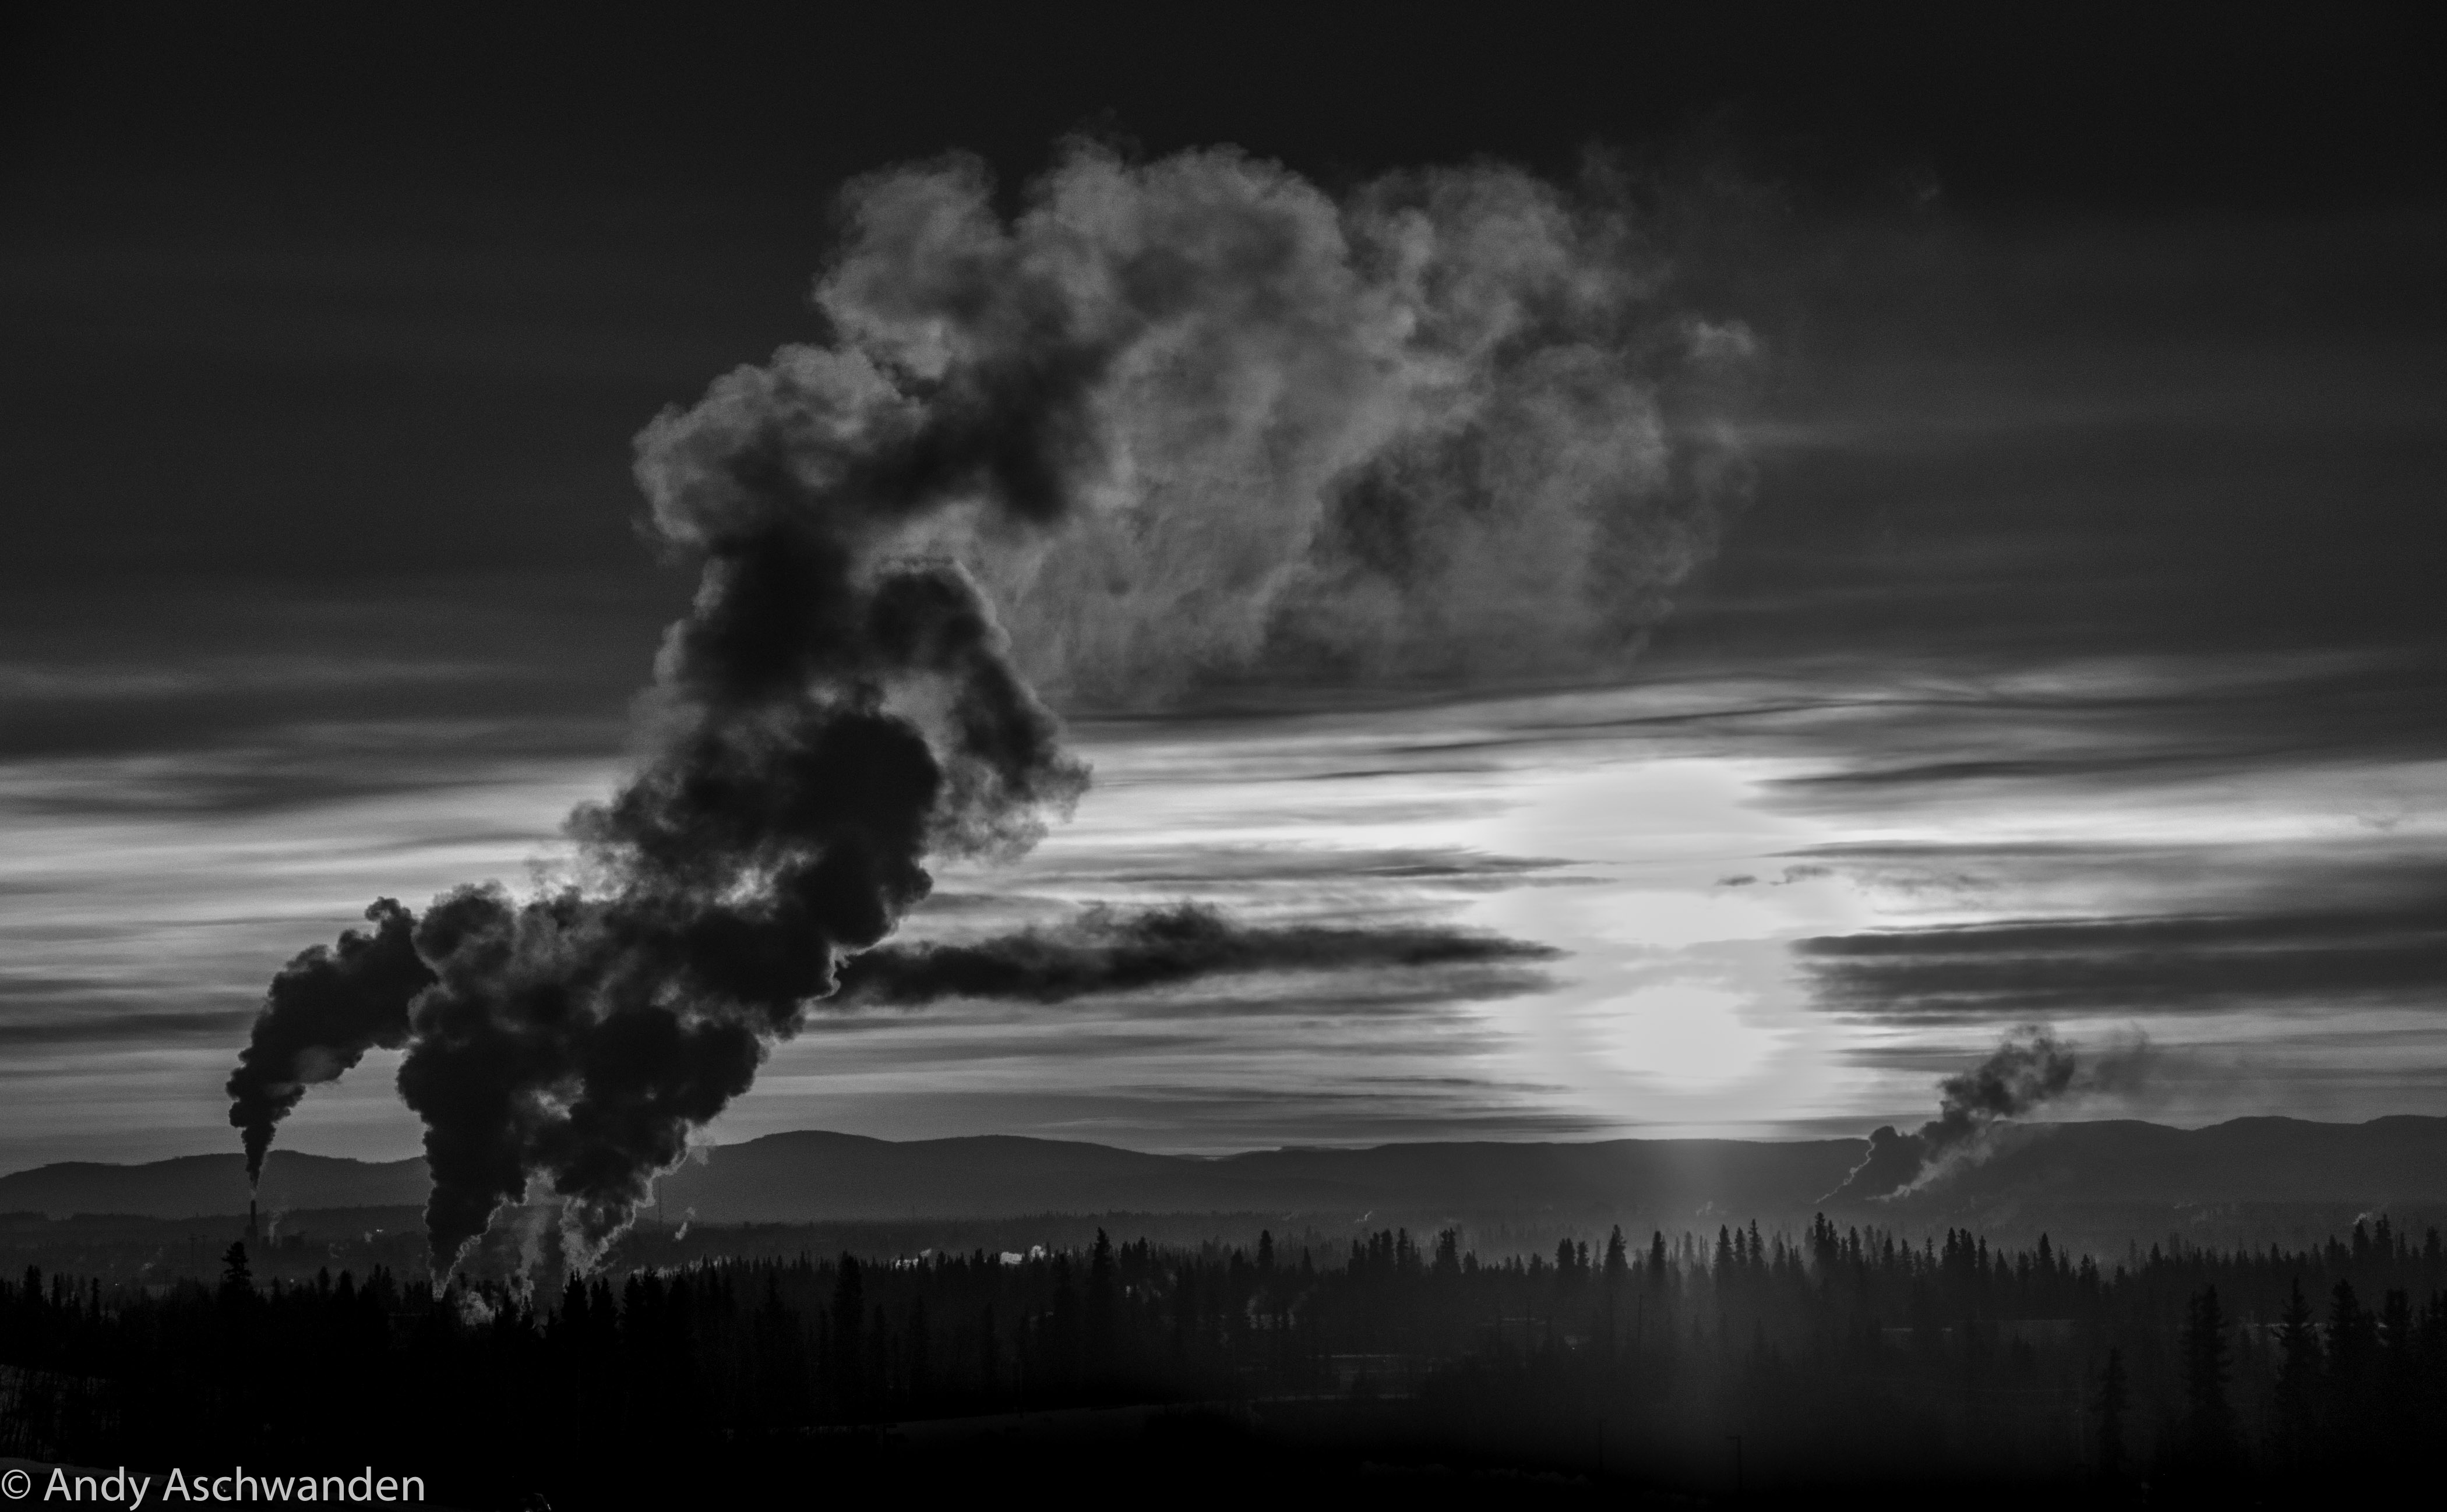
\includegraphics[height=\paperheight,width=\paperwidth]{uaf_power_plant}};}
} 

\begin{frame}{What if this trend continues?}
    \begin{itemize}
      \item Combustion of available fossil fuel resources sufficient to eliminate the Antarctic Ice Sheet (Winkelmann \emph{et al.}, 2015)
      \item and probably the  Greenland Ice Sheet too
      \item though this would take on the order of 10,000 years
    \end{itemize}
    \note[item]{Where is the carbon dioxide coming from}
  \note[item]{Now that we know carbon dioxide is driving temperture changes}
  \note[item]{where will this lead to?}
  \note[item]{CO2 is produced by burning of fossil fuels}
  \note[item]{My colleagues asked the a provocative question: what would happen if\ldots}
\end{frame}

\setbeamertemplate{background canvas}
  {
} 

\begin{frame}{What does this mean}
  \begin{figure}
    \includegraphics<1>[width=\textwidth]{sea-level-potential-simple-01}
    \includegraphics<2>[width=\textwidth]{sea-level-potential-liberty-01}
  \end{figure}
  \note[item]{How much ice can we melt?}
  \note<1>[item]{If all glaciers melted, sea level would rise by 1 meter}
  \note<1>[item]{If the Greenland Ice Sheet melted, sea level would rise by 6 meter (or 20ft)}
  \note<1>[item]{If the Greenland Ice Sheet melted, sea level would rise by 6 meter (or 20ft)}
  \note[item]{All the glaciers of Alaska, Switzerland, Himalaya, etc.}
\end{frame}


% \setbeamertemplate{background canvas}
%   {
%      \tikz{\node[inner sep=0pt,opacity=1] {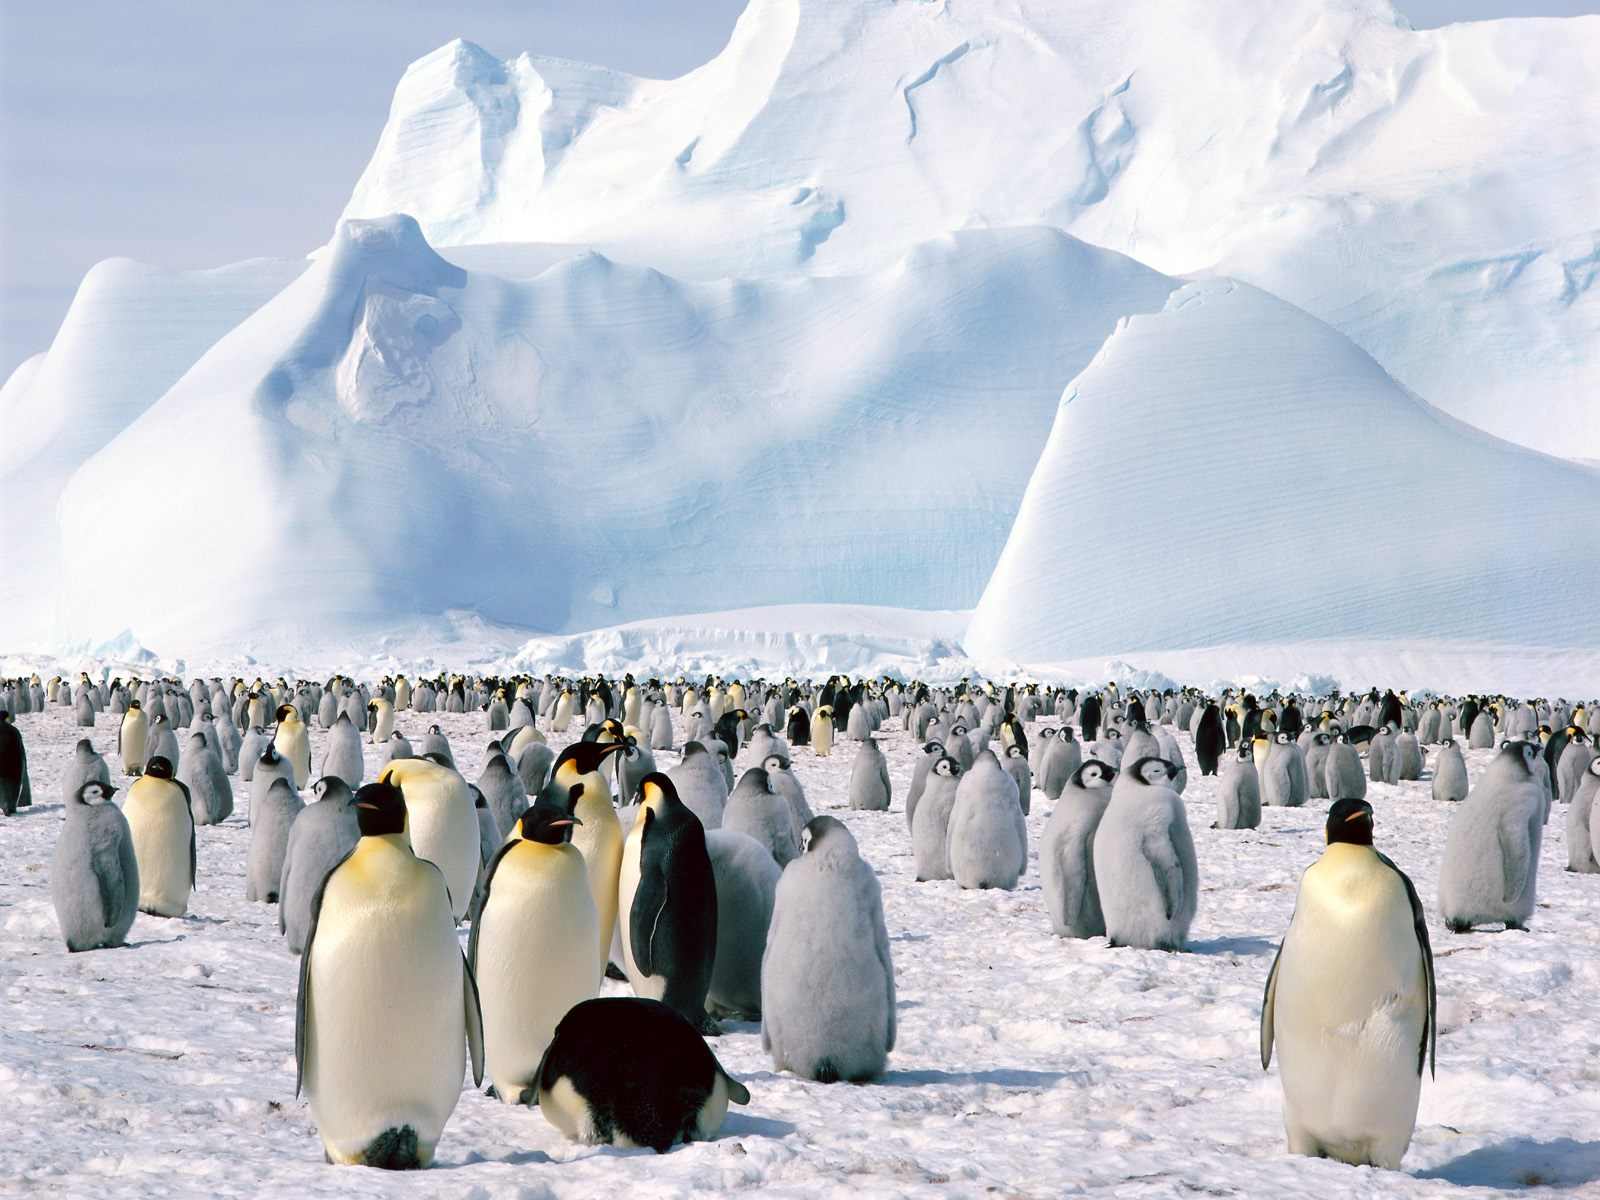
\includegraphics[height=\paperheight,width=\paperwidth]{ant_penguins}};}
% } 

% \begin{frame}[plain]
% \end{frame}

% \setbeamertemplate{background canvas}
%   {
%      \tikz{\node[inner sep=0pt,opacity=1] {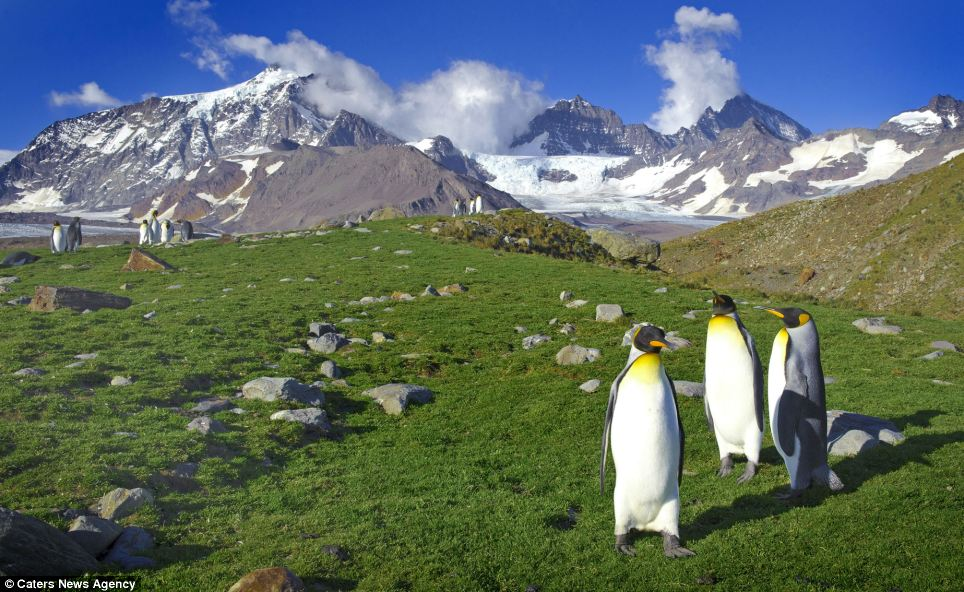
\includegraphics[height=\paperheight,width=\paperwidth]{green_penguins}};}
% } 



\begin{frame}[plain]
How realistic is that?
\end{frame}

\setbeamertemplate{background canvas}
  {
     \tikz{\node[inner sep=0pt,opacity=1] {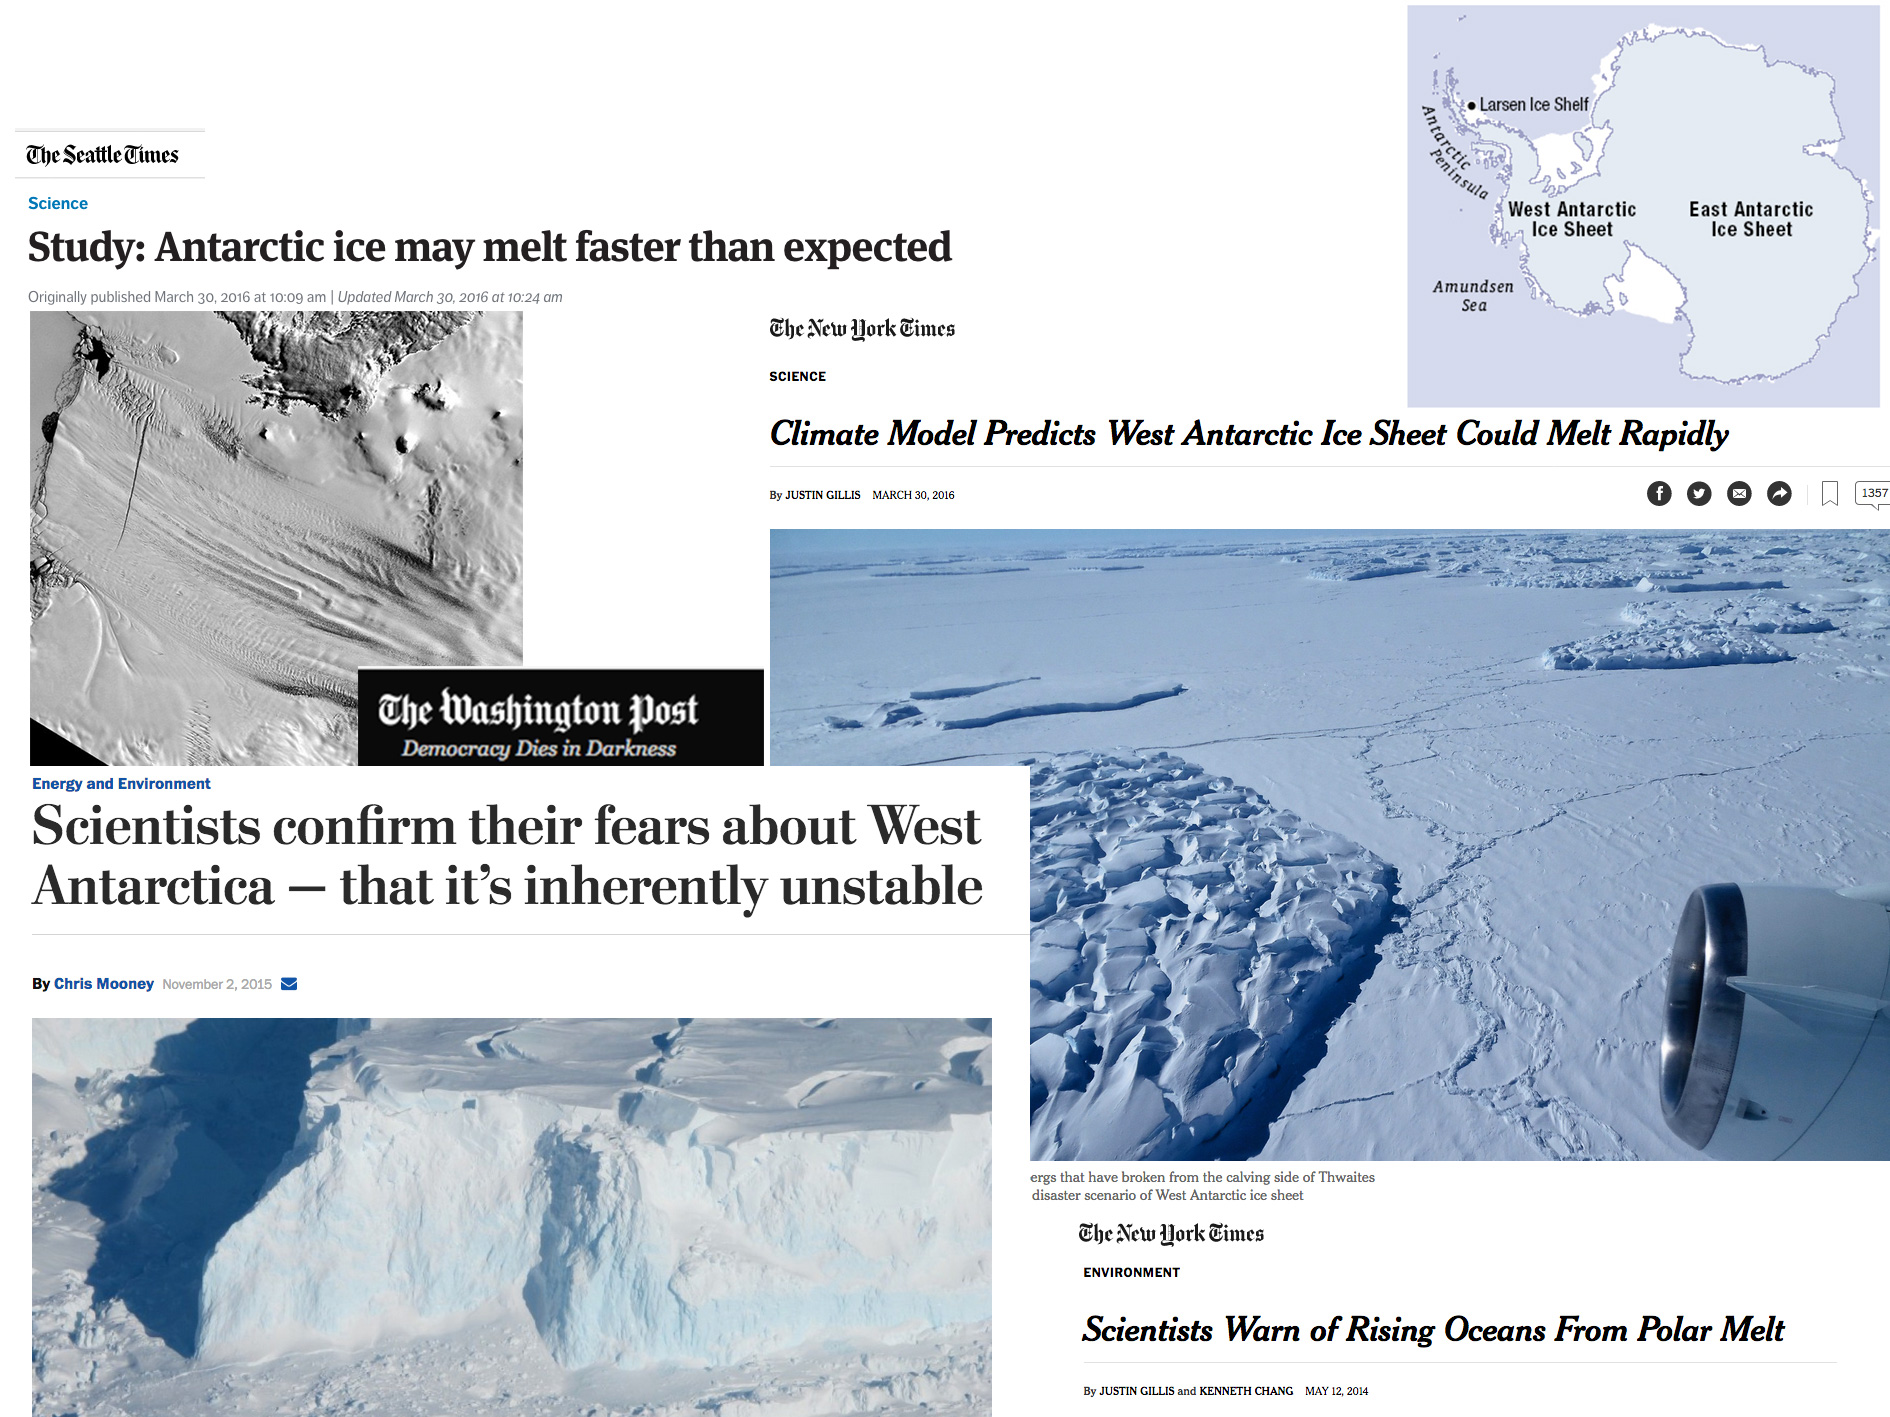
\includegraphics[height=\paperheight,width=\paperwidth]{wais-news}};}
} 

\begin{frame}{Antartica in the News}
  \note[item]{In the past 2--3 years, West Antartica has been in the news frequently}
  \note[item]{Explain where West Antartica is, ice shelf scales}
\end{frame}

\setbeamertemplate{background canvas}
  {
} 

\begin{frame}{Antartica The Continent}
  \begin{figure}
    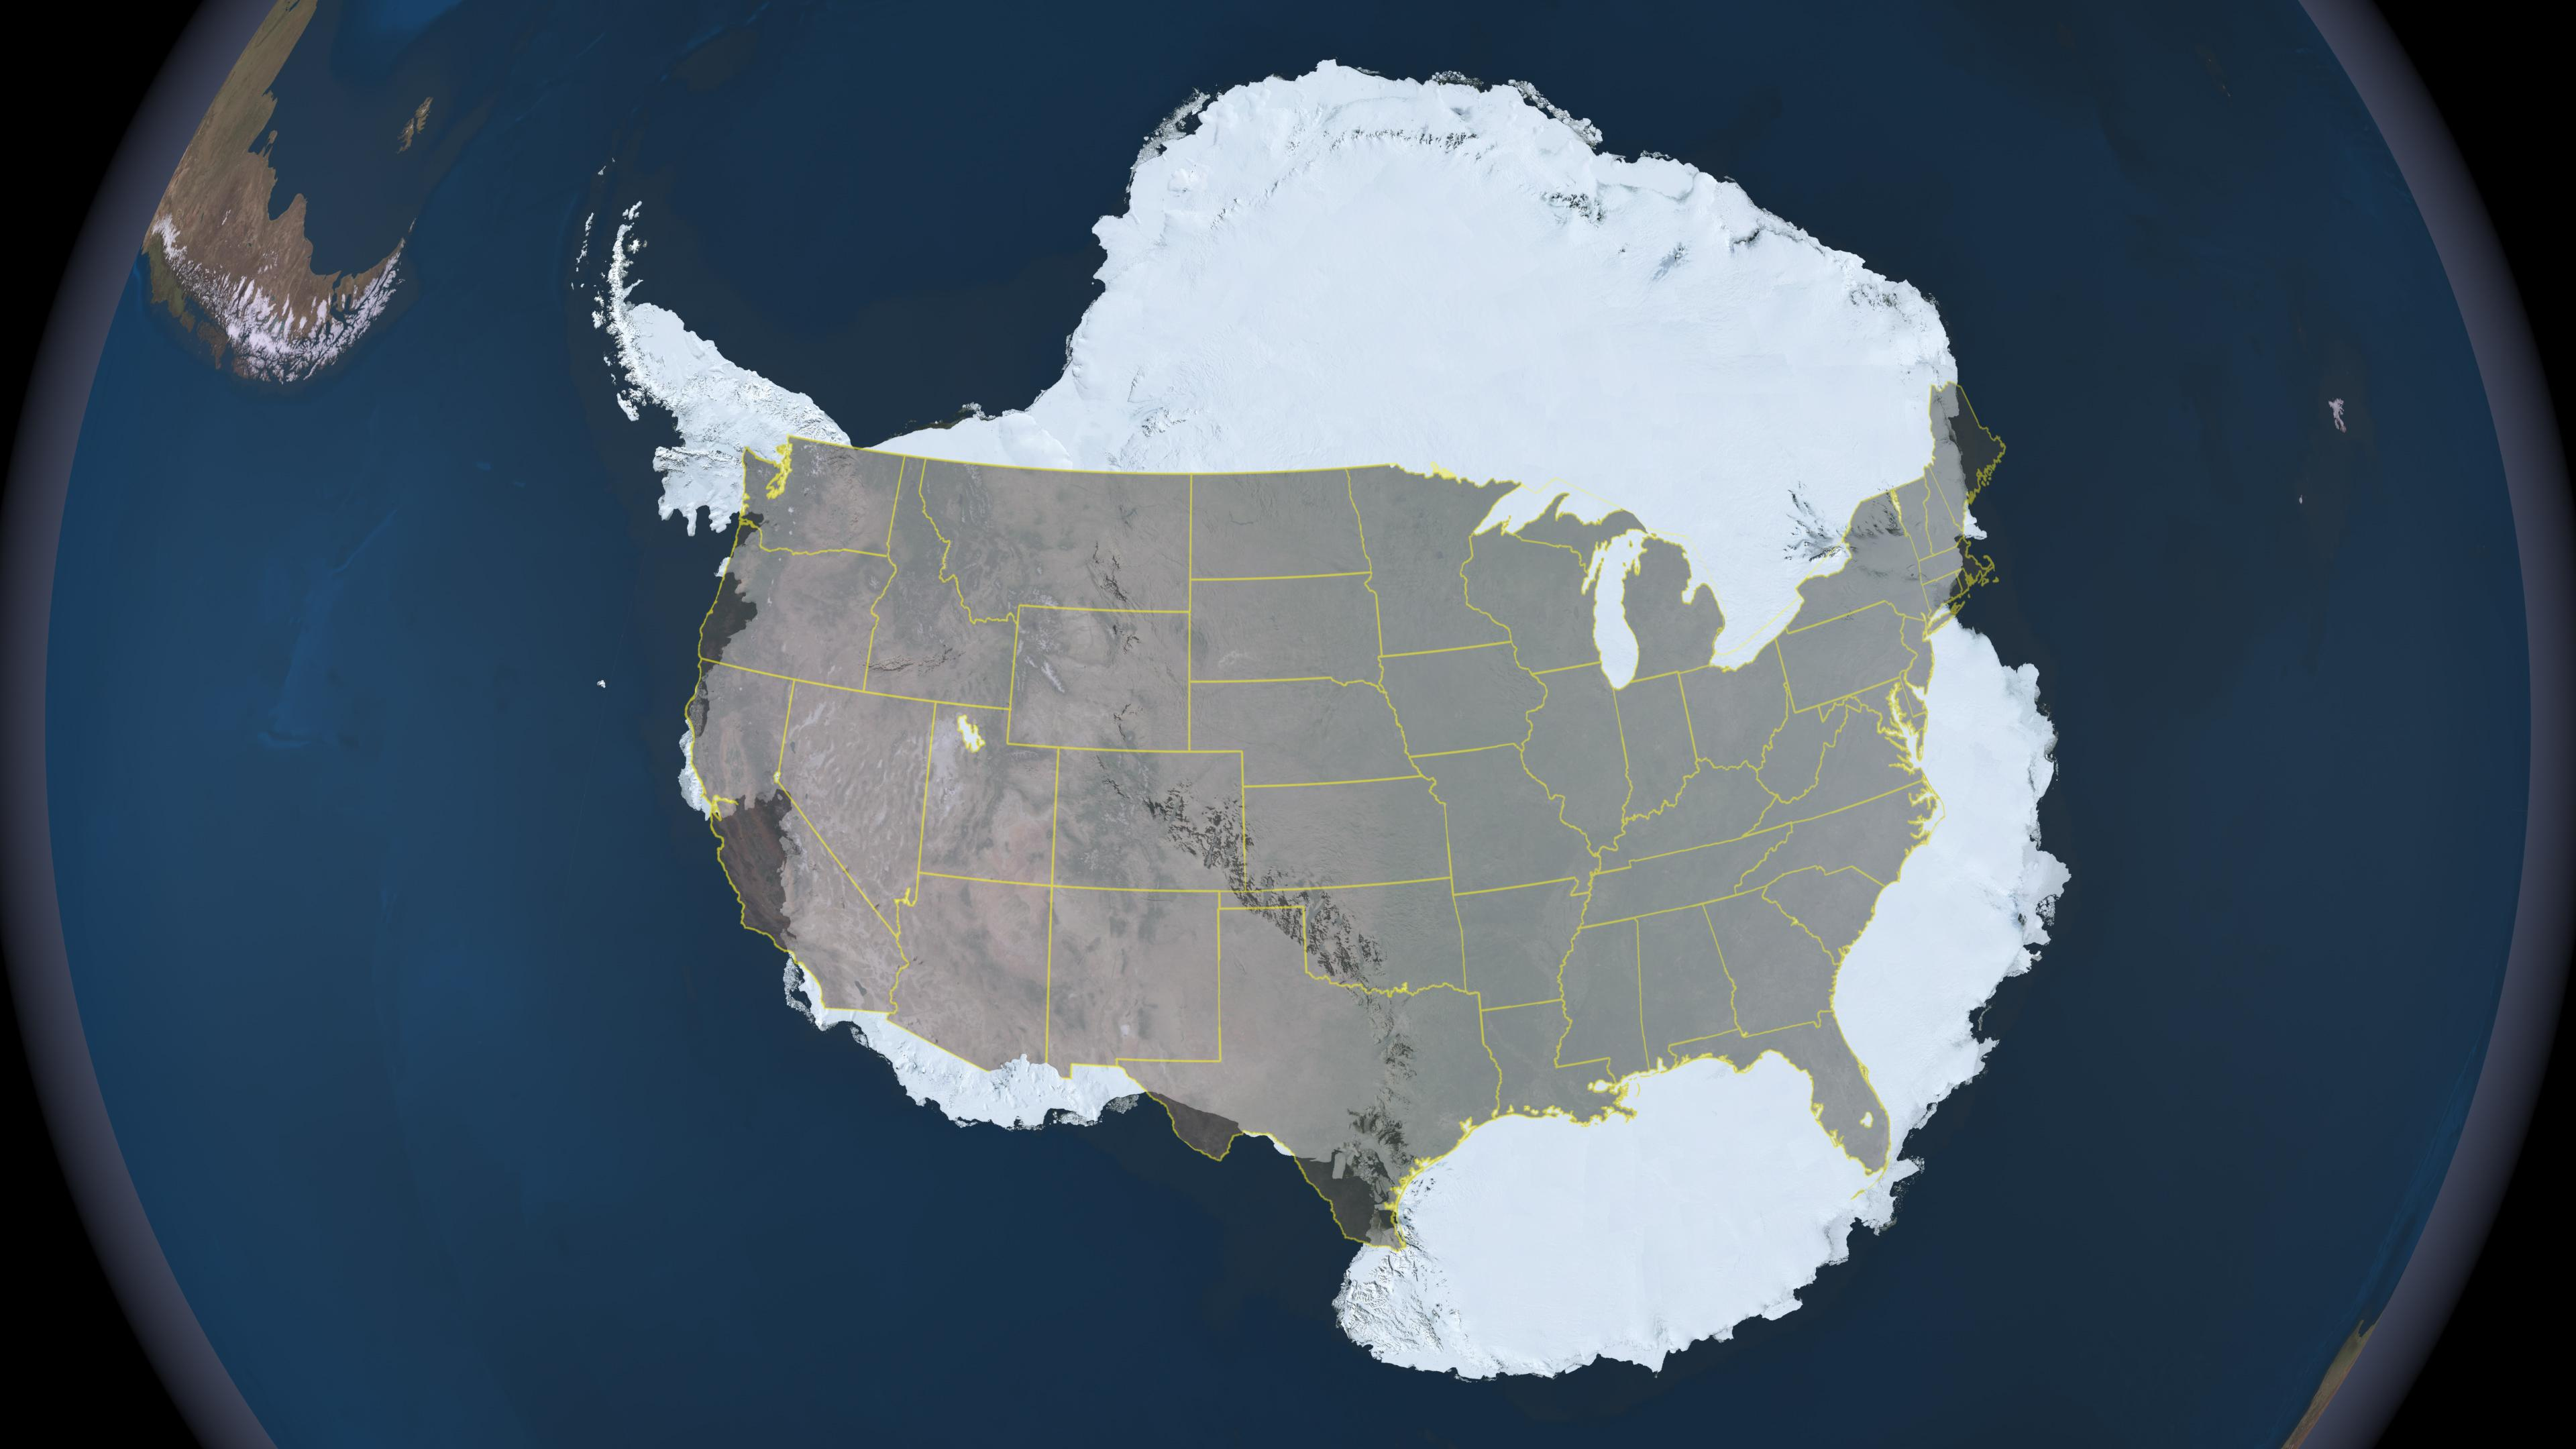
\includegraphics[width=\paperwidth]{main_USA_Antarctica_size}
  \end{figure}
  \note{
  Antarctica is the highest, driest, coldest, windiest and brightest of the seven continents. It is roughly the size of the United States and Mexico combined and is almost completely covered by a layer of ice that averages more than one mile in thickness, but is nearly three miles thick in places. This ice accumulated over millions of years through snowfall. Presently, the Antarctic ice sheet contains 90\% of the ice on Earth}
\end{frame}

\begin{frame}{Antartica The Continent}
  \begin{figure}
    \includegraphics[width=\paperwidth]{ant-ice-shelf-map}
  \end{figure}
\end{frame}


\setbeamertemplate{background canvas}
{
} 


% \begin{frame}{How an alpine glacier works}
%   \begin{figure}
%     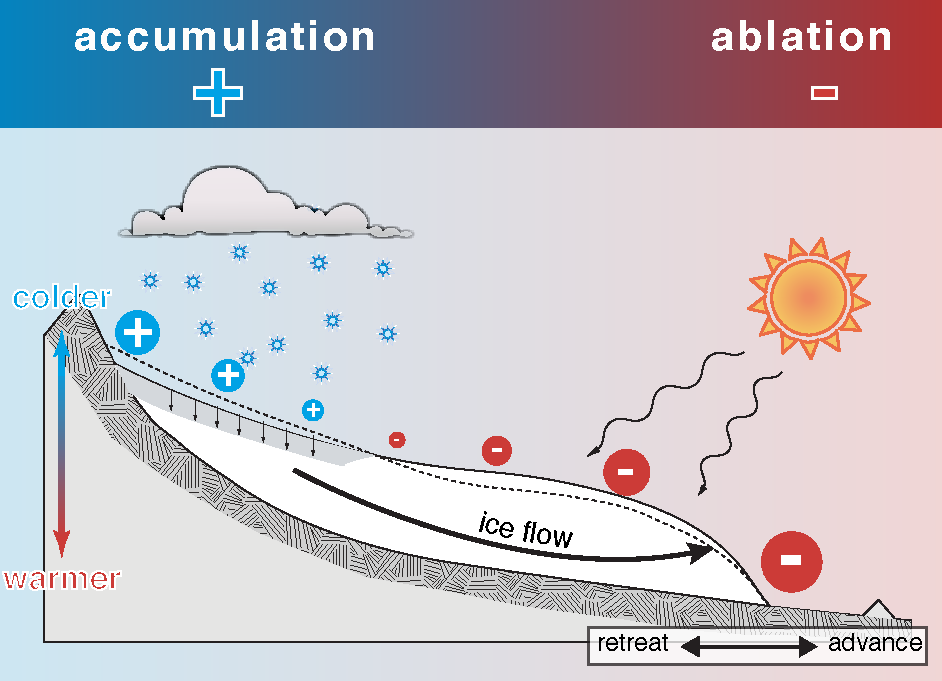
\includegraphics[width=.98\textwidth]{glacier_mb}
%   \end{figure}
%   \note[item]{in general, the higher up we go, the colder it gets}
%   \note[item]{though this is not always true in Fairbanks}
%   \note[item]{as those of you living up in the hills appreciate}
%   \note[item]{snow accumulates in the colder, higher altitude areas in the interior}
%   \note[item]{turns into ice}
%   \note[item]{and starts to flow downhill towards the coast}
%   \note[item]{this is basically the definition of a glacier}
%   \note[item]{a large chunk of ice the moves under its own weight}
%   \note[item]{there's an initmate relationship between temperature and the health of glaciers}
%   \note[item]{glaciers are sensitive to air temperature}
% \end{frame}


\begin{frame}{The Antartic Ice Sheet}
  \begin{figure}
    \includegraphics<1>[width=\textwidth]{ice-sheet-cartoon-simple}
    \includegraphics<2>[width=\textwidth]{ice-sheet-cartoon-simple-box}
  \end{figure}
  \note[item]{Most of the ice rests on land}
  \note[item]{but xxx floats}
  \note[item]{difference between shelf and land base: floating and friction}
\end{frame}


\begin{frame}{Antartica The Continent}
  \begin{figure}
    \includegraphics[width=\paperwidth]{ant-ice-shelf-map}
  \end{figure}
\end{frame}


\begin{frame}{Marine Ice Sheet Instability Hypothesis}
 \begin{figure}
  \movie[showcontrols=true,width=10cm]{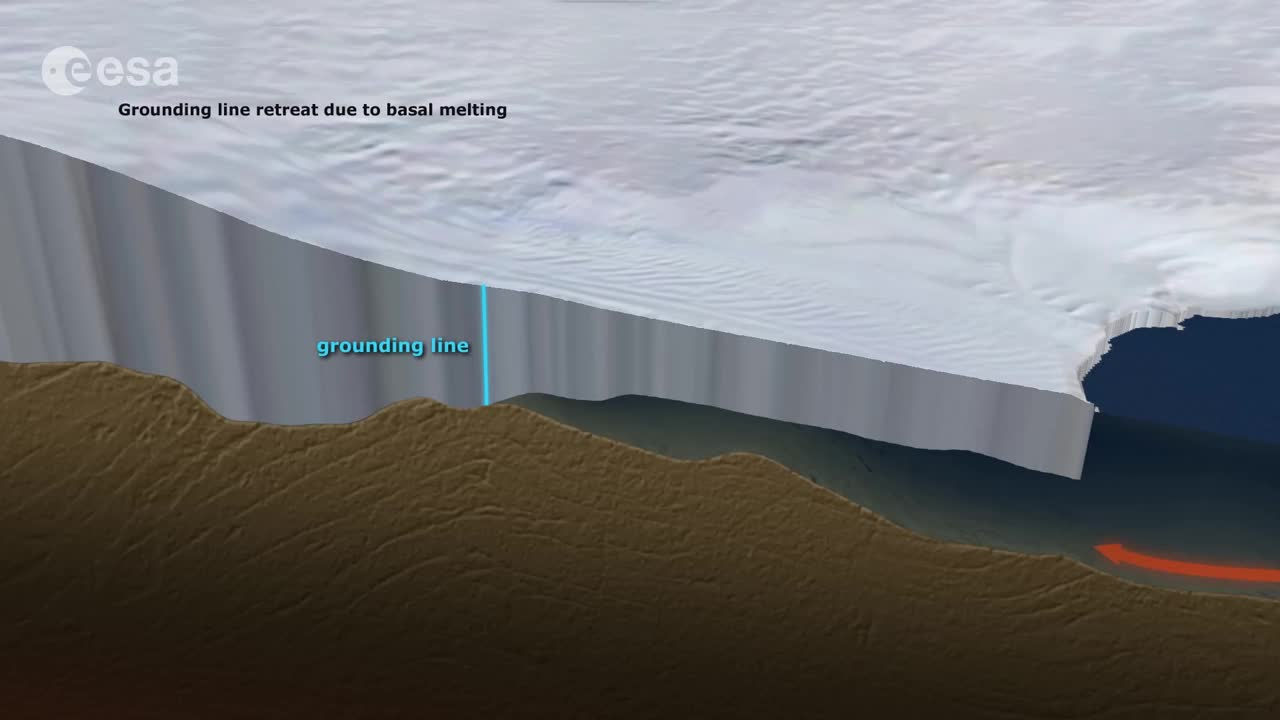
\includegraphics[width=10cm]{gl-retreat}}{gl-retreat.mov}
  \end{figure}
  \note[item]{attacked from underneath}
  Antartica is a desert. ice shelf attack
  n\note[item]{water is more effective, how to thaw moose meat}
  \note[item]{once it passes the grounding line, it has contributed to sea level}
\end{frame}


\begin{frame}{Marine Ice Sheet Instability Hypothesis}
  \begin{columns}[c]
    \begin{column}{.65\linewidth}
      \begin{figure}
        \includegraphics<1>[height=8cm]{ant-marine}
      \end{figure}
    \end{column}
    \begin{column}{.38\linewidth}
      \begin{itemize}
      \item blue colors: below sea level
      \end{itemize}
    \end{column}
  \end{columns}
\end{frame}

\begin{frame}{West Antarctic Ice Sheet}
  \movie[showcontrols=true,width=10cm]{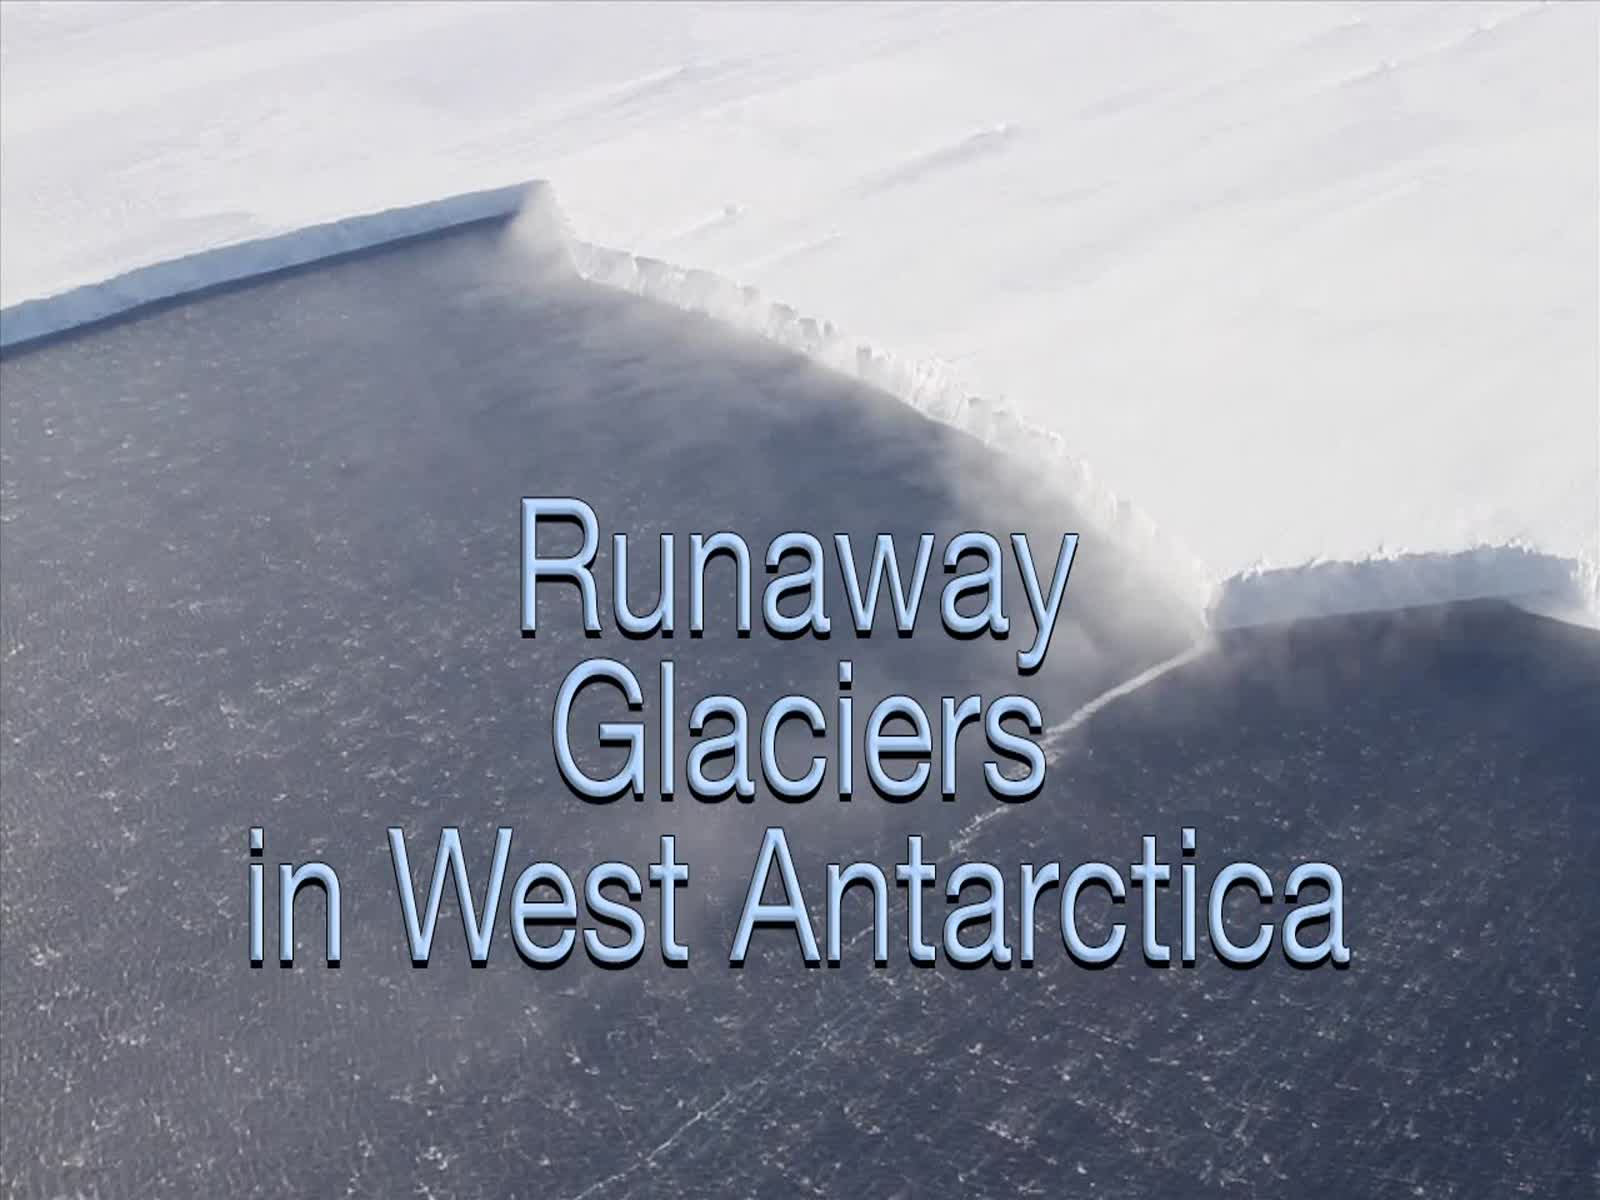
\includegraphics[width=10cm]{rignot-wais}}{rignot-wais.mov}
\end{frame}

\begin{frame}{The Latest Results}
  Pollard and DeConto (2016)
  \begin{itemize}
  \item 1 meter by 2100
  \item 6 meter by 2500
  \end{itemize}
Why is this so important. Why understand what's going on top, but will happen underneath. That's 
\end{frame}


\begin{frame}{The biggest losers might be us}
\begin{itemize}
\item 40 percent of the world's population lives within 62 miles (100 kilometers) of the ocean, putting millions of lives and billions of dollars' worth of property and infrastructure at risk. 
\item we already dealt with this
\end{itemize}
\end{frame}

% \setbeamertemplate{background canvas}
% {
%   \tikz{\node[inner sep=0pt,opacity=1] {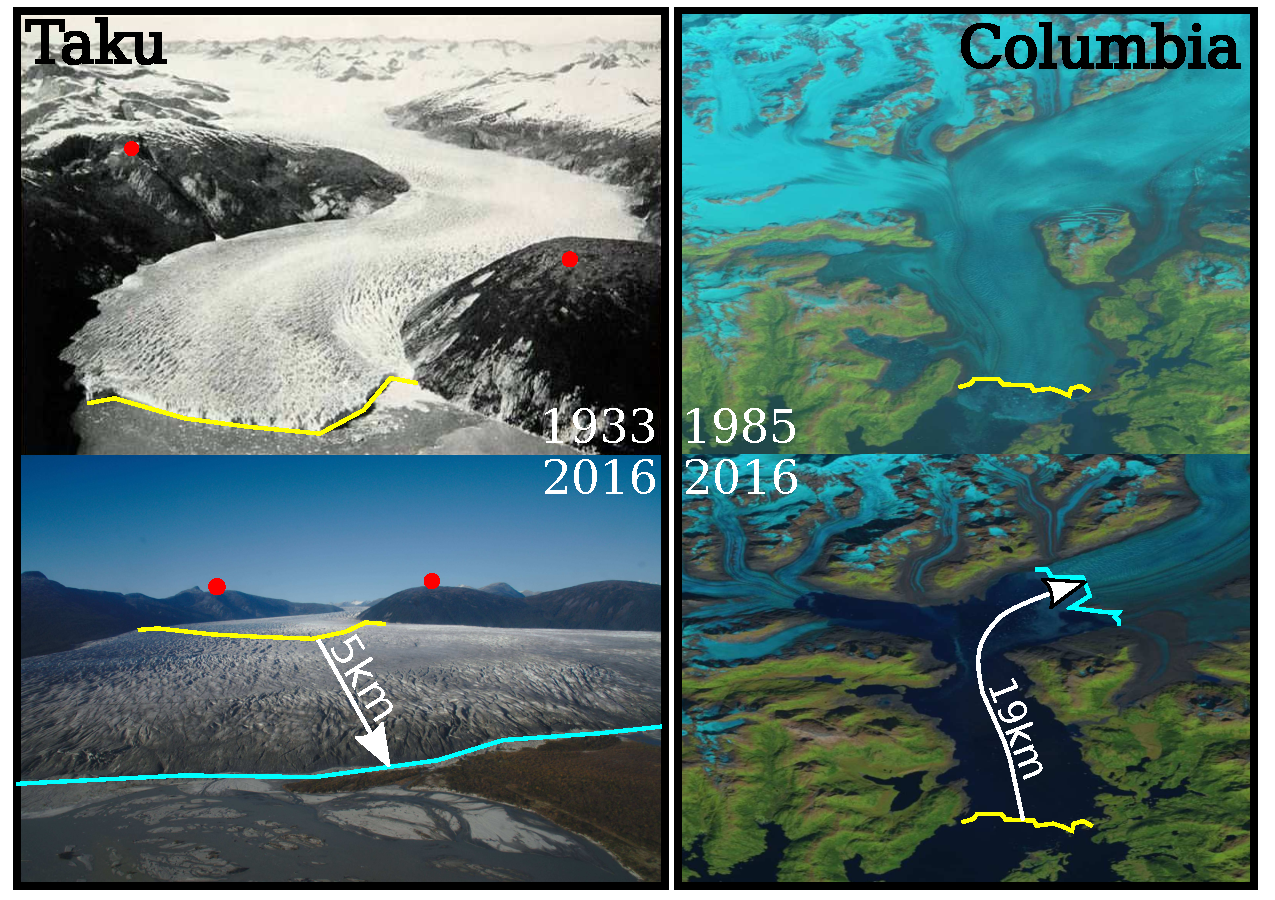
\includegraphics[height=\paperheight,width=\paperwidth]{brinkerhoff-collage}};}
% }

% \begin{frame}[plain]
% \note[item]{I would like end this presentation with a more positive note}
% \note[item]{Ship taku}
% \end{frame}

% \setbeamertemplate{background canvas}
% {
% }

% \begin{frame}{Sediment Transport Drives Tidewater Glacier Periodicity}
%   \begin{figure}
%   \movie[showcontrols=true,width=10cm]{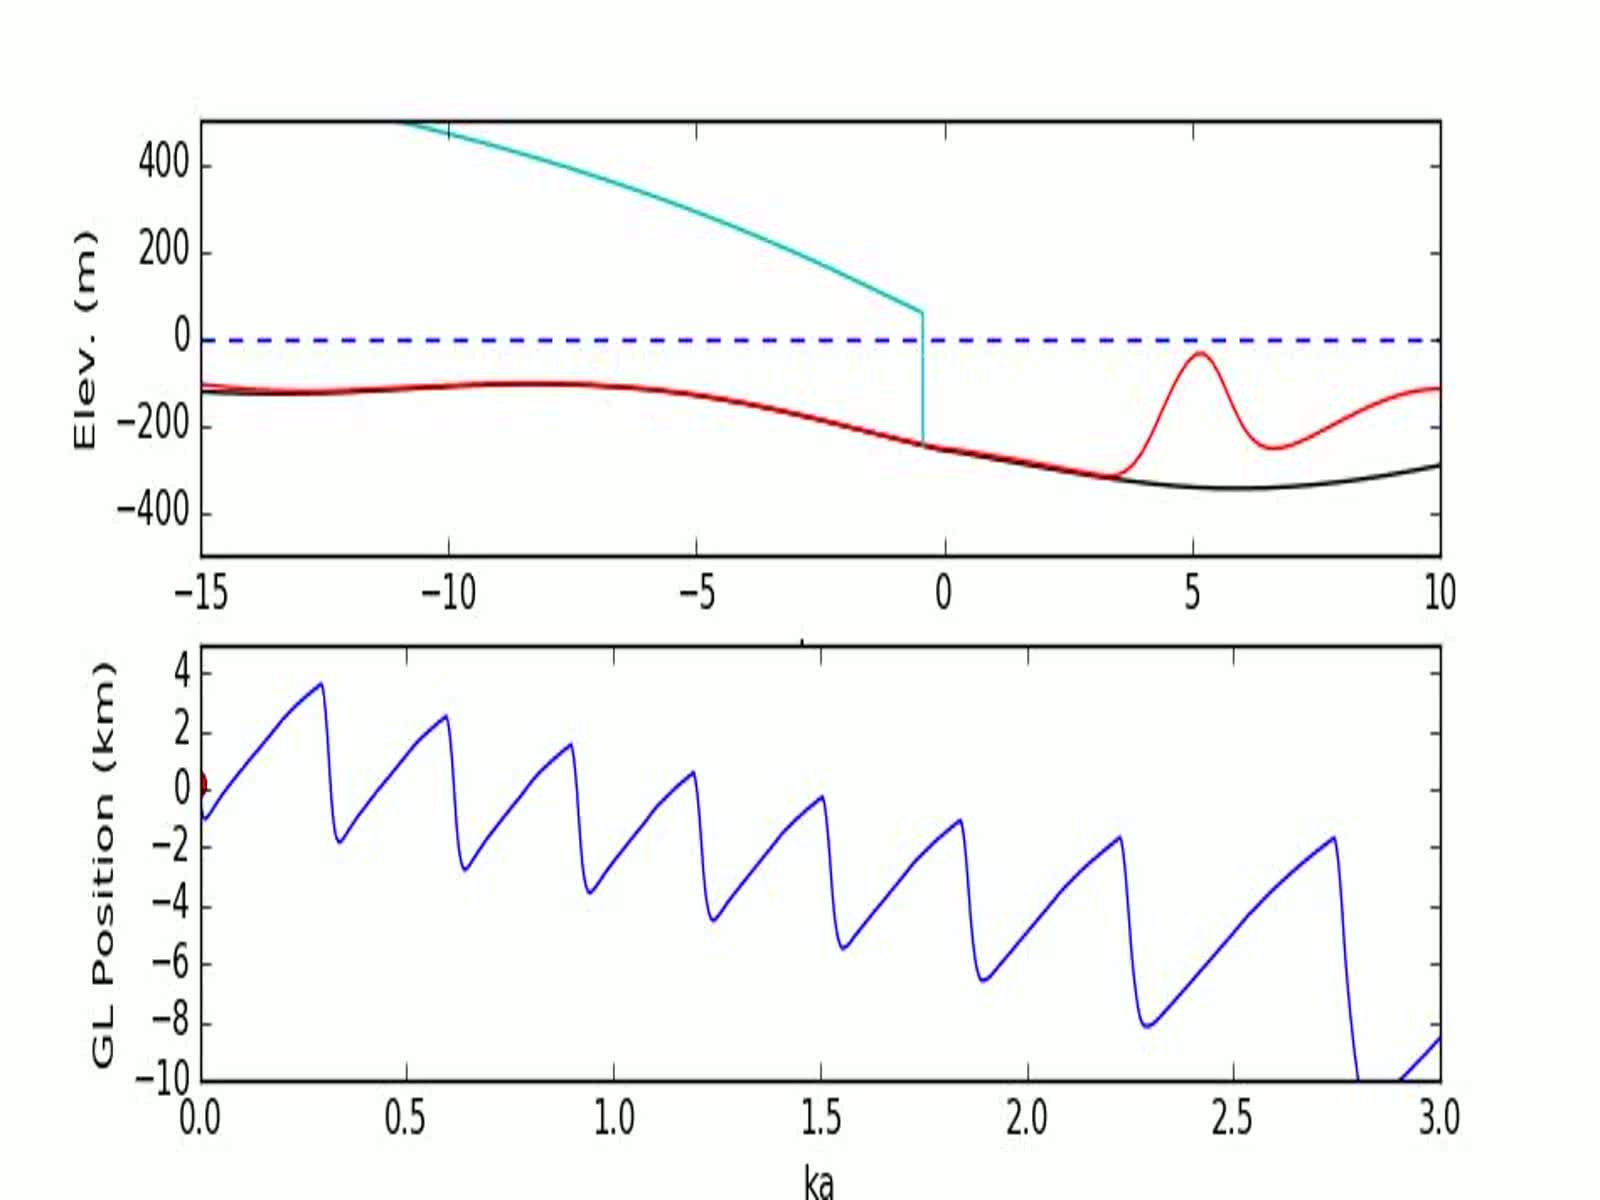
\includegraphics[width=10cm]{tidewater-glacier}}{tidewater-glacier.mov}
%   {\\ D. Brinkhoff (UAF)}
% \end{figure}
% \end{frame}

\setbeamertemplate{background canvas}
{
  \tikz{\node[inner sep=0pt,opacity=1] {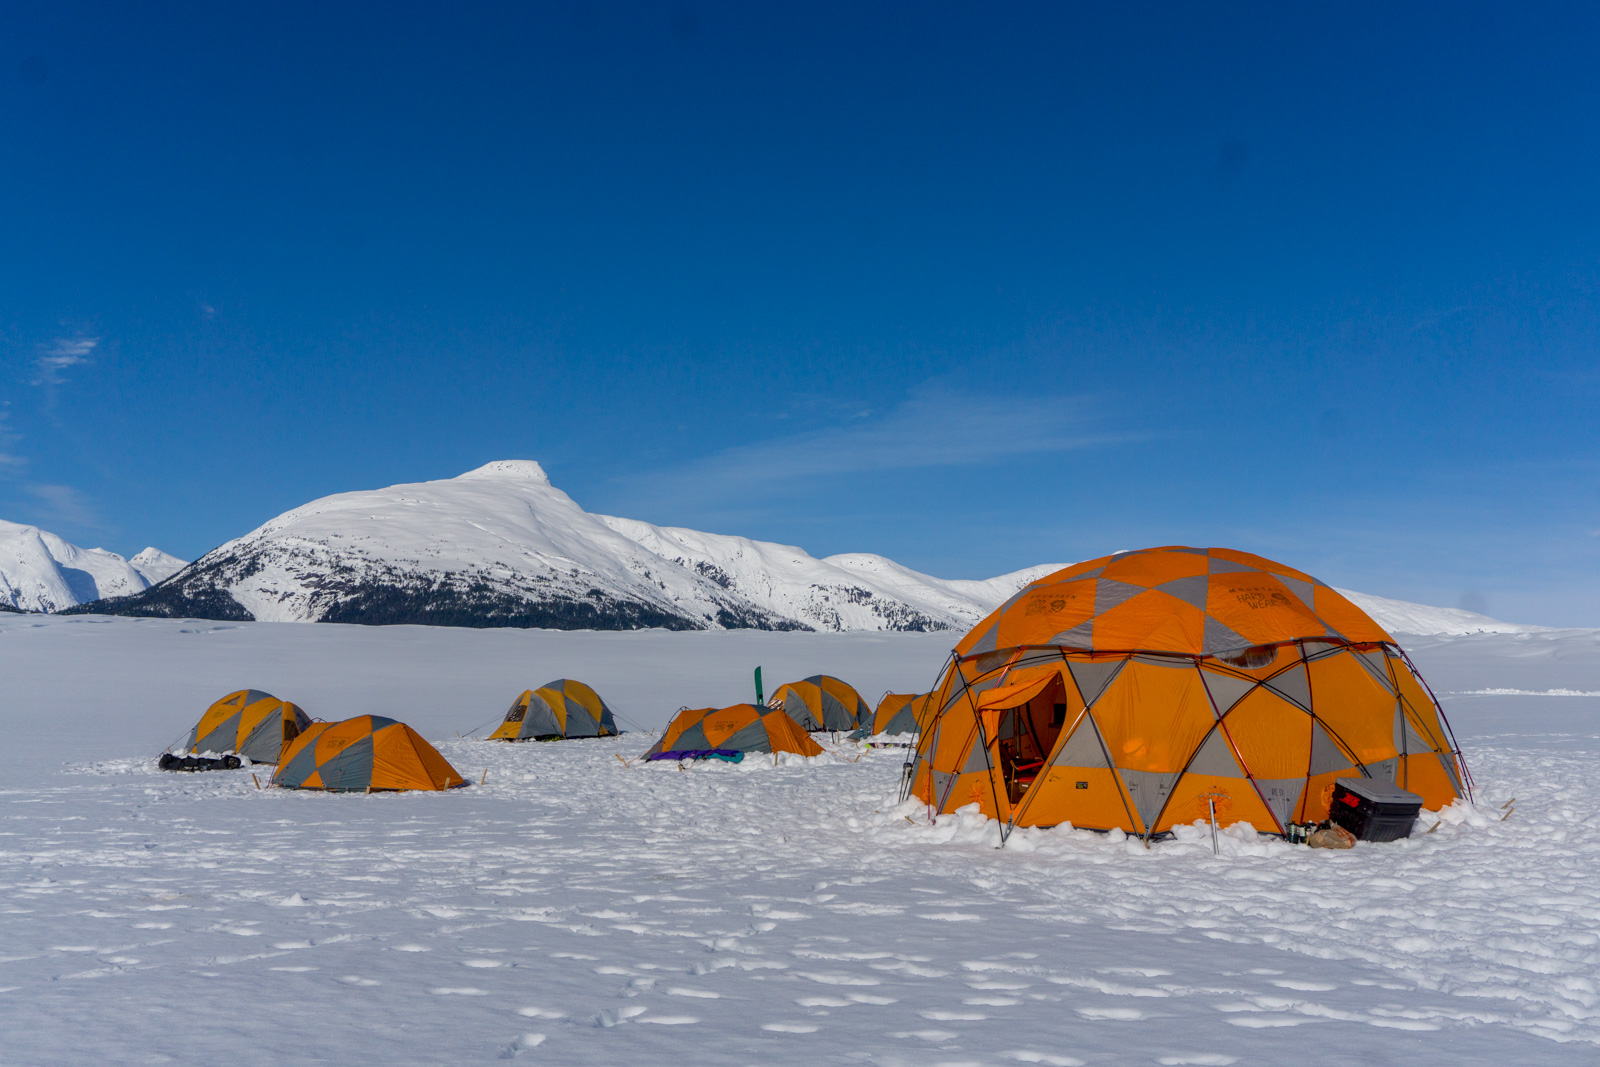
\includegraphics[height=\paperheight,width=\paperwidth]{taku-8}};}
}

\begin{frame}{Questions?}

\end{frame}

\setbeamertemplate{background canvas}
{
}

\begin{frame}{The sun drives the glacial/interglacial cycle}
  \vspace{-2cm}
  \begin{block}{Milankovitch Cycle}
    \begin{figure}
      \movie[showcontrols=true,autostart,loop,width=8cm]{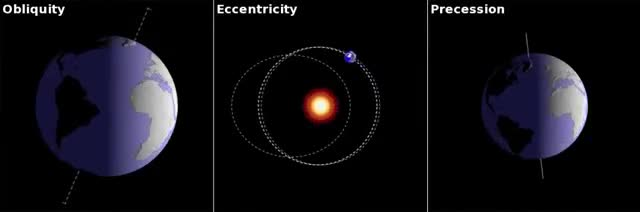
\includegraphics[width=8cm]{orbital-forcing}}{orbital-forcing.mov}
    \end{figure}
  \end{block}
  \begin{columns}[T]
    \begin{column}{.32\linewidth}
      41,000 yrs
    \end{column}
    \begin{column}{.32\linewidth}
      100,000 yrs
    \end{column}
    \begin{column}{.32\linewidth}
      26,000 yrs
    \end{column}
  \end{columns}
  \note[item]{Changes in the obliquity (tilt) of Earth's axis}
  \note[item]{Variations in the shape of Earth's orbit (eccentricity)}
  \note[item]{Changes in Earth's "Wobble" (Precession)}
  \note[item]{ When less solar energy is received earth enters into an ice age; when earth begins to receive more solar energy it comes out of the ice age. The amount of solar energy and the resulting changes to temperature this has can be worked out and it amounts to around 5 degrees C.}
  \note[item]{The additional rise and fall in temperatures beyond the 5 degrees C range can only be explained by the effects of CO2 concentration in the atmosphere due to various feedback or forcing mechanisms.}
  \note[item]{As the earth's temperature begins to drop feedback occur that reduce the amount of CO2 being produced and atmospheric concentrations begin to fall.}
  \note[item]{At the end of an ice age as more solar energy is received and again as temperatures begin to rise; feedbacks begin to produce more CO2 increasing CO2 concentrations.}
\end{frame}


\begin{frame}
    \begin{figure}
      \movie[showcontrols=true,loop,width=10cm]{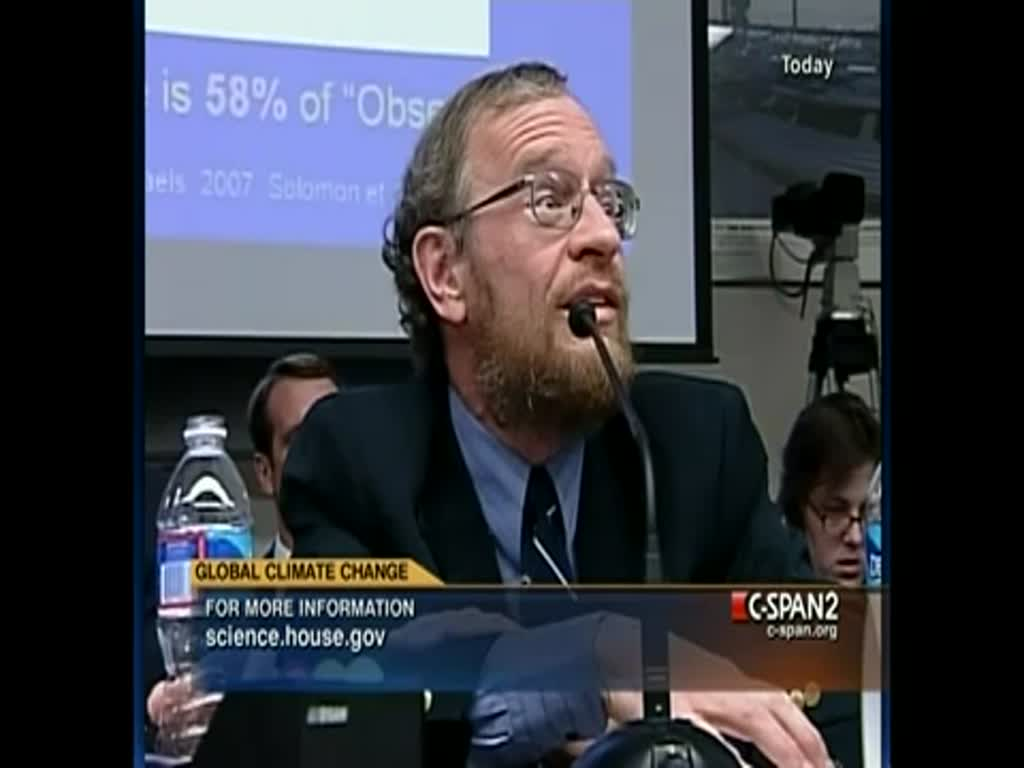
\includegraphics[width=10cm]{alley-001}}{alley-milankovitch.mov}
    \end{figure}
    \note[item]{My colleague Richard Alley is much more eqloquent in explain what causes ice ages}
    \note[item]{as he did in this hearing in front of congress a couple of years ago}
\end{frame}

\begin{frame}{The Greenhouse Effect\ldots{}is not rocket science}
  \begin{itemize}
  \item The existence of the greenhouse effect was argued for by Joseph Fourier in 1824.
  \item The argument and the evidence were further strengthened by Claude Pouillet in 1827 and 1838 
  \item and reasoned from experimental observations by John Tyndall in 1859, who measured the radiative properties of specific greenhouse gases.
  \item The effect was more fully quantified by Svante Arrhenius in 1896, who made the first quantitative prediction of global warming due to a hypothetical doubling of atmospheric carbon dioxide
  \end{itemize}
\end{frame}

\begin{frame}{Carbon Dioxide}
      \begin{figure}
        \includegraphics<1>[width=\textwidth]{nasa_co2-graph}
      \end{figure}
\end{frame}


\end{document}

